%% Auteur: Simon-Pierre Boucher, Université Laval, Chapitre 2 : thèse de doctorat

\documentclass[12pt]{article}

\usepackage{amssymb,amsmath,amsfonts,eurosym,geometry,ulem,graphicx,caption,color,setspace,comment,footmisc,pdflscape,subfigure,array,hyperref}
\usepackage{rotating}
\usepackage{multirow}
\usepackage{tabularx}
\usepackage{booktabs}
\usepackage{lscape}
\usepackage[dvipsnames]{xcolor}
\definecolor{mypink1}{rgb}{0.858, 0.188, 0.478}
\usepackage{tablefootnote}
\usepackage{ragged2e}
\usepackage{nicematrix}
\usepackage{enumitem}
\usepackage{wasysym}
\usepackage{framed}
\usepackage{pgfgantt}
\usepackage{subfloat}
\usepackage{blindtext}
\usepackage{colortbl}
\usepackage{palatino}
\usepackage{mathpazo}
\usepackage[flushleft]{threeparttable}
\usepackage[margin=15pt,font=small,labelfont={bf,sf}]{caption}
\usepackage[semibold]{sourcesanspro}
\usepackage{sectsty}
\allsectionsfont{\sffamily}

\hypersetup{colorlinks,
citecolor=blue,
linkcolor=magenta
}

\usepackage{environ,atbegshi}
\makeatletter
\newif\ifAtEnd@DontShowMe
\newcommand*\contents@DontShowMe{}

\normalem

\doublespacing
\newtheorem{theorem}{Theorem}
\newtheorem{corollary}[theorem]{Corollary}
\newtheorem{proposition}{Proposition}
\newenvironment{proof}[1][Proof]{\noindent\textbf{#1.} }{\ \rule{0.5em}{0.5em}}

\newtheorem{hyp}{Hypothesis}
\newtheorem{subhyp}{Hypothesis}[hyp]
\renewcommand{\thesubhyp}{\thehyp\alph{subhyp}}

\usepackage{natbib}
\bibliographystyle{chicago}%abbrvnat
\setcitestyle{authoryear,open={(},close={)}} %Citation-related commands
\geometry{left=1.0in,right=1.0in,top=1.0in,bottom=1.0in}
\title{\textbf{Modelling Volatility Dynamics Between Commodity ETFs and Their Net Asset Value using BVAR and HAR Models}%\thanks{The authors thank participants at seminars at Humboldt University Berlin, South Dakota State University (Ness School), University of Illinois, Urbana-Champaign (ACE), and at meetings of the Commodity \& Energy Markets Association (2021),  World Finance \& Banking Association (2021), Société canadienne de science  économique (2022), 4th Ethical Finance and Sustainability (EFS) conference (2022), and Multinational Finance Society (2022), as well as Jocelyn Grira, Joseph Marks, Alessandro Melone (discussants) and Scott Irwin,  Michel Robe and Zhiguang Wang. For financial support, the authors thank the Social Sciences and Humanities Research Council and the Chaire Industrielle-Alliance Groupe financier. Any remaining errors are ours alone.}
}


\author{Simon-Pierre Boucher\footnote{PhD student in finance, Université Laval, Quebec City QC Canada G1V 0A6, email:   \texttt{simon-pierre.boucher.1@ulaval.ca}}\and Marie-H{\'e}l{\`e}ne Gagnon\footnote{Professor of Finance and Research Fellow, CRREP, Université Laval, email: \texttt{marie-helene.gagnon@fsa.ulaval.ca}}\and Gabriel J. Power\footnote{IG Wealth Management Chairholder, Professor of Finance and Research Fellow, CRREP and CRIB, Université Laval, email:   \texttt{gabriel.power@fsa.ulaval.ca}}}

\date{\today}
\begin{document}
\begin{titlepage}
\maketitle

\begin{abstract}
\singlespacing
\noindent 
We examine volatility transmission between commodity ETFs and their underlying assets using high-frequency realized variance data across multiple sampling frequencies. Analyzing crude oil, gold, silver, and natural gas ETFs with HAR-X models and Bayesian VAR, we document systematic heterogeneity in volatility spillovers. Precious metals exhibit strong unidirectional transmission from underlying assets to ETFs, with gold coefficients reaching 0.632 at 1-minute frequency and negligible reverse effects. Energy commodities show bidirectional transmission with asymmetries favoring underlying-to-ETF spillovers. Sampling frequency critically affects transmission measurement: 1-minute data reveals effects up to three times larger than 30-minute estimates. Jump components dominate continuous volatility transmission, particularly for precious metals. Our Bayesian analysis confirms that underlying volatility often rivals ETF self-persistence in predicting ETF dynamics. 

\vspace{0.2in}
\noindent\textbf{Keywords:} ETF volatility transmission, commodity markets, realized variance, HAR models, market microstructure.\\
\textbf{JEL Classification:} G12, G13, G14, C32

\bigskip
\end{abstract}
\doublespacing

\setcounter{page}{0}
\thispagestyle{empty}
\end{titlepage}
\pagebreak \newpage




% Include all sections
%% Auteur: Simon-Pierre Boucher, Université Laval, Chapitre 2 : thèse de doctorat

\section{Introduction} 
The global exchange-traded fund (ETF) market has experienced remarkable growth over the past two decades, with assets under management exceeding \$10 trillion by 2023 \citep{petajisto2017inefficiencies}.  Within this landscape, commodity ETFs have emerged as increasingly important financial instruments, providing investors with accessible exposure to commodity markets without the complexities of direct futures trading or physical storage \citep{gorton2006facts}. These instruments have fundamentally altered the structure of commodity markets, introducing new channels for price discovery and volatility transmission that warrant careful empirical investigation.

The theoretical foundation for understanding ETF pricing rests on the arbitrage mechanism that links ETF prices to their underlying Net Asset Values (NAVs). Under ideal market conditions, authorized participants (APs) ensure that ETF prices remain closely aligned with their NAVs through creation and redemption processes \citep{ackert2000arbitrage}. However, this mechanism may become less effective during periods of market stress, when liquidity constraints and trading costs can lead to persistent deviations from fundamental values \citep{madhavan2012exchange}. The resulting price dynamics create complex volatility transmission patterns between ETFs and their underlying assets that have important implications for market efficiency and risk management.

Despite the growing importance of commodity ETFs, our understanding of high-frequency volatility dynamics between these instruments and their underlying assets remains limited. While extensive research exists on equity ETFs \citep{ben2018etfs, israeli2017etf}, and some studies examine commodity ETF tracking performance \citep{todorov2021etf}, few investigations focus specifically on the intraday volatility spillover mechanisms that characterize these markets. This gap is particularly significant given that commodity markets exhibit distinct characteristics—including seasonal patterns, storage constraints, and supply disruptions—that may generate unique volatility transmission dynamics.

This study addresses these limitations by conducting a comprehensive analysis of volatility dynamics in commodity ETF markets using high-frequency data and advanced econometric techniques. We construct indicative Net Asset Value (iNAV) series for four major commodity ETFs—representing gold (GLD), silver (SLV), crude oil (USO), and natural gas (UNG)—using minute-by-minute pricing data over a 13-year period from 2010 to 2023. Our methodological approach combines Heterogeneous Autoregressive (HAR) models, which capture the long-memory characteristics of realized volatility \citep{corsi2009simple}, with Bayesian Vector Autoregression (BVAR) techniques that accommodate time-varying interdependencies while addressing overfitting concerns \citep{koop2011forecasting}.

Our research questions are structured around testable hypotheses that contribute to the literature regardless of empirical outcomes. First, we examine whether volatility transmission between commodity ETFs and their iNAVs exhibits bidirectional relationships versus unidirectional patterns. Second, we investigate whether high-frequency sampling reveals volatility transmission mechanisms that are obscured in traditional daily analysis. Third, we test whether different commodity types—precious metals versus energy commodities—exhibit systematically different volatility transmission patterns. Finally, we assess whether the iNAV serves merely as a passive reflection of underlying asset movements or functions as an active determinant of ETF volatility.

Our empirical findings reveal significant heterogeneity in volatility transmission patterns across commodity types and sampling frequencies. For precious metals ETFs (GLD and SLV), we document predominantly unidirectional spillovers from iNAV to ETF, with coefficients ranging from 0.35 to 0.63 in our HAR specifications. Energy commodity ETFs (USO and UNG) exhibit bidirectional transmission, though with stronger effects flowing from iNAV to ETF markets. High-frequency (1-minute) sampling captures substantially stronger daily effects compared to lower frequencies, while weekly and monthly components remain stable across sampling intervals. These patterns are robust across both HAR and BVAR frameworks, with impulse response functions confirming rapid shock absorption and asymmetric adjustment mechanisms.

This study makes several important contributions to the literature. Methodologically, we are the first to construct comprehensive high-frequency iNAV series for commodity ETFs over an extended time period, enabling detailed analysis of intraday market dynamics. Empirically, we document systematic differences in volatility transmission mechanisms across commodity types, providing new insights into the role of underlying asset characteristics in determining ETF market behavior. From a practical perspective, our findings have important implications for risk management strategies, suggesting that monitoring underlying asset volatility is particularly crucial for precious metals ETFs, while energy ETF markets require attention to bidirectional feedback effects.

For investors, our results suggest that volatility forecasting models for commodity ETFs should incorporate high-frequency information from underlying assets, particularly for short-term trading strategies. For regulators, the documented asymmetries in volatility transmission indicate that oversight approaches may need to be tailored to different commodity types, with particular attention to the potential for amplified volatility effects in precious metals markets. For market makers and authorized participants, our findings highlight the importance of understanding frequency-dependent arbitrage opportunities and the varying effectiveness of price discovery mechanisms across different commodity sectors.

The remainder of this paper is structured as follows. Section 2 reviews the relevant literature on ETF pricing mechanisms, volatility transmission, and commodity market dynamics. Section 3 describes our data construction methodology and presents descriptive statistics. Section 4 outlines our econometric framework, including HAR and BVAR model specifications. Section 5 presents our empirical results, and Section 6 concludes with implications for theory and practice.

%% Auteur: Simon-Pierre Boucher, Université Laval, Chapitre 2 : thèse de doctorat

\section{Literature Review} \label{sec:literature}

This section provides a comprehensive review of the theoretical and empirical literature relevant to volatility transmission in commodity ETF markets. We organize our discussion around five key themes: the theoretical foundations of ETF arbitrage mechanisms, the empirical evidence on ETF impact on underlying asset markets, the development of high-frequency volatility measurement and modeling techniques, the specific characteristics of commodity markets and their financialization, and the emerging literature on ETF market microstructure during crisis periods. This comprehensive framework allows us to identify critical gaps in existing knowledge and precisely position our contribution within the broader literature on ETF market dynamics and volatility transmission.

\subsection{Theoretical Foundations of ETF Arbitrage Mechanisms}

The theoretical underpinnings of ETF pricing rest fundamentally on the arbitrage relationship between ETF shares and their underlying Net Asset Values, first rigorously analyzed by \citet{ackert2000arbitrage}. Their seminal framework demonstrates that authorized participants (APs) can create or redeem ETF shares in exchange for baskets of underlying securities, theoretically ensuring price alignment through arbitrage. This mechanism relies on the assumption that arbitrageurs can costlessly and instantaneously exploit price discrepancies, maintaining the no-arbitrage condition that ETF prices equal their fundamental values.

However, the theoretical elegance of this framework faces significant challenges in practice. \citet{pontiff1996costly} provides early theoretical insights into the limits of arbitrage, showing that transaction costs, capital constraints, and noise trader risk can prevent arbitrageurs from eliminating pricing anomalies. These insights prove particularly relevant for ETF markets, where authorized participants face substantial operational complexities and regulatory constraints.

\citet{gromb2010limits} extend this theoretical framework by examining how funding liquidity affects arbitrage effectiveness. Their model demonstrates that when arbitrageurs face binding capital constraints, price deviations can persist even when arbitrage opportunities are clearly identified. This theoretical insight has profound implications for ETF pricing, particularly during periods of market stress when authorized participants may face increased margin requirements and reduced access to funding.

The theoretical literature has also examined the role of market makers in ETF pricing. \citet{hendershott2013relationship} develop a model showing that market makers' inventory management concerns can create systematic patterns in ETF pricing errors. When market makers accumulate large inventory positions, they adjust quotes to encourage trades that reduce their exposure, potentially creating persistent deviations from NAV. This theoretical framework helps explain why ETF pricing errors may exhibit predictable patterns related to trading volume and market volatility.

Recent theoretical advances have focused on the feedback effects between ETF trading and underlying asset markets. \citet{malamud2016portfolio} develop a general equilibrium model demonstrating that ETF trading can affect the volatility and correlation structure of underlying assets through portfolio rebalancing effects. Their model shows that when ETFs experience large flows, the resulting trades in underlying assets can create systematic volatility spillovers that persist beyond the initial shock.

\citet{ben2017etfs} provide a comprehensive theoretical framework for understanding how ETFs affect price discovery in underlying markets. Their model demonstrates that ETFs can both enhance and impede price discovery, depending on the relative efficiency of ETF and underlying asset markets. When ETF markets are more liquid and efficient, they can serve as venues for informed trading that ultimately improves price discovery in underlying assets. Conversely, when ETF trading is dominated by uninformed flow, it can inject noise into underlying asset prices.

The theoretical literature has also examined the specific challenges facing commodity ETFs. \citet{basak2016model} develop a model of commodity financialization that demonstrates how financial trading through commodity ETFs can increase price volatility and reduce the correlation between prices and fundamental supply and demand factors. Their model shows that when financial traders dominate commodity markets, prices can deviate substantially from fundamental values, creating complex volatility transmission patterns.

\subsection{Empirical Evidence on ETF Market Efficiency and Pricing}

The empirical literature examining ETF market efficiency presents mixed evidence on the effectiveness of arbitrage mechanisms. \citet{petajisto2017inefficiencies} provides the most comprehensive analysis of ETF pricing efficiency using data on over 1,000 U.S. ETFs from 2000 to 2015. He documents significant and persistent pricing deviations, with median absolute deviations from NAV averaging 40 basis points for bond ETFs and 15 basis points for equity ETFs. Importantly, these deviations are not randomly distributed but exhibit systematic patterns related to fund characteristics, market conditions, and underlying asset liquidity.

\citet{shin2013basis} examine the determinants of ETF pricing errors using a comprehensive sample of international equity ETFs. They find that pricing errors are significantly related to underlying market volatility, ETF trading volume, and the liquidity of underlying assets. Their results suggest that arbitrage effectiveness deteriorates precisely when it is most needed—during periods of high volatility and market stress.

The role of authorized participants in maintaining ETF pricing efficiency has received considerable empirical attention. \citet{dannhauser2017effect} examines how the number and identity of authorized participants affects ETF pricing. Using detailed data on AP activity, she finds that ETFs with more authorized participants exhibit smaller and less persistent pricing errors. However, she also documents that during periods of market stress, even ETFs with multiple APs can experience significant pricing dislocations.

\citet{pan2016etf} provide compelling evidence on how liquidity mismatches between ETFs and underlying assets affect arbitrage effectiveness. Using the 2014-2015 Russian financial crisis as a natural experiment, they show that when underlying assets become illiquid, ETFs can trade at substantial premiums or discounts to NAV for extended periods. During the peak of the crisis, some Russian equity ETFs traded at discounts exceeding 20\% of NAV for several weeks.

The empirical literature has also examined ETF pricing during extreme market events. \citet{madhavan2012exchange} provides a detailed analysis of ETF behavior during the May 6, 2010 flash crash. He documents that many ETFs experienced severe price dislocations, with some trading at discounts exceeding 40\% of NAV. Importantly, these dislocations were not randomly distributed but were concentrated among ETFs holding less liquid underlying assets and those with fewer authorized participants.

\citet{staer2017asset} extends this analysis by examining ETF behavior during multiple crisis episodes, including the 2008 financial crisis, the 2010 European sovereign debt crisis, and the 2015 Chinese stock market crash. She finds that ETF pricing errors increase systematically during crisis periods, with the magnitude of errors related to underlying asset illiquidity and the complexity of the ETF structure.

Recent empirical work has focused on the high-frequency dynamics of ETF pricing. \citet{richie2008examination} examine intraday price relationships between the SPDR S\&P 500 ETF (SPY) and its underlying index using tick-by-tick data. They find evidence of rapid price discovery, with ETF prices adjusting to new information within minutes. However, they also document systematic patterns in pricing errors related to market opening and closing effects.

\citet{hasbrouck2003intraday} extends this analysis to examine price discovery across multiple ETFs and their underlying assets. Using vector error correction models applied to high-frequency data, he finds that price discovery is shared between ETF and underlying asset markets, with the relative contribution varying based on trading volume and market conditions. His results suggest that ETFs serve as important venues for price discovery, particularly during periods of high market activity.

\subsection{ETF Impact on Underlying Asset Markets: Price Discovery and Volatility}

The growing prominence of ETFs has fundamentally altered the microstructure of underlying asset markets, with important implications for price discovery and volatility transmission. The empirical literature has produced competing findings on whether ETFs enhance or impede market efficiency, reflecting the complex nature of these relationships.

\citet{glosten2021etf} provide strong evidence that ETFs enhance price discovery in underlying assets. Using comprehensive data on ETF trading and underlying stock prices, they show that ETF order flow contains significant information about future stock returns. They estimate that ETF trading accounts for approximately 15\% of total price discovery in large-cap stocks, with this contribution increasing during periods of high market volatility. Their findings suggest that ETFs serve as efficient aggregation mechanisms for broad market information.

However, \citet{ben2018etfs} present compelling counter-evidence suggesting that ETFs may increase non-fundamental volatility in underlying assets. Using a comprehensive sample of U.S. stocks from 1993 to 2012, they find that stocks with higher ETF ownership exhibit 15-20\% higher return volatility, even after controlling for fundamental volatility measures. This effect is particularly pronounced for stocks held by multiple ETFs, suggesting that ETF-driven correlations create systematic volatility spillovers across securities.

\citet{israeli2017etf} extend this analysis by examining how ETF ownership affects information production and processing in underlying markets. They find that stocks with higher ETF ownership receive less analyst coverage and exhibit weaker relationships between accounting fundamentals and stock prices. These findings suggest that while ETFs may improve market-level price discovery, they may simultaneously reduce security-specific information production.

The impact of ETFs on underlying asset liquidity represents another contested area in the literature. \citet{hamm2014liquidity} documents that increased ETF ownership is associated with reduced liquidity in individual stocks, as measured by wider bid-ask spreads and higher price impact measures. She argues that this occurs because traders substitute ETF trading for individual stock trading, reducing the flow of stock-specific information and decreasing market maker incentives to provide liquidity in individual securities.

Conversely, \citet{agarwal2018etfs} find that ETFs generally improve liquidity in underlying assets by attracting additional trading interest and providing more efficient price discovery mechanisms. Using a comprehensive sample of U.S. equity ETFs, they show that stocks with higher ETF ownership exhibit lower transaction costs and higher trading volume. They argue that ETFs create positive externalities by attracting uninformed traders who provide liquidity to informed traders.

The resolution of this apparent contradiction may lie in the heterogeneity of ETF effects across different market segments and time periods. \citet{krause2014exchange} examine ETF effects across different market capitalization segments, finding that ETFs improve liquidity for large-cap stocks but may reduce liquidity for small-cap stocks. They argue that this reflects the fixed costs of maintaining ETF arbitrage relationships, which make arbitrage less profitable for smaller, less liquid stocks.

Recent empirical work has examined the dynamic nature of ETF effects on underlying markets. \citet{da2018exchange} show that the impact of ETFs on underlying asset correlations varies significantly over time, with stronger effects during periods of market stress. They find that ETF-driven correlations increase substantially during crisis periods, potentially amplifying systemic risk and reducing diversification benefits.

\citet{broman2016liquidity} provide evidence on the style-investing effects of ETFs, showing that ETFs can create excess comovement among stocks with similar characteristics. Using data on sector and style ETFs, they demonstrate that stocks held by the same ETFs exhibit higher return correlations, even after controlling for fundamental similarities. This excess comovement represents a source of non-fundamental volatility that can persist for extended periods.

\subsection{High-Frequency Volatility Measurement and Modeling}

The development of realized variance measures using high-frequency data represents one of the most significant advances in financial econometrics over the past two decades. This literature provides the methodological foundation for our analysis of volatility transmission in ETF markets.

\citet{andersen2001distribution} provide the seminal contribution to this literature, demonstrating that realized variance computed from high-frequency returns provides nearly unbiased estimates of integrated volatility. Using comprehensive data on individual stocks and market indices, they show that 5-minute realized variance measures substantially outperform traditional volatility proxies based on daily data. Their work establishes the statistical properties of realized variance and demonstrates its superiority for volatility forecasting applications.

\citet{barndorff2002econometric} extend this framework by providing rigorous asymptotic theory for realized variance estimators. They demonstrate that as the sampling frequency increases, realized variance converges to integrated volatility under general conditions. Importantly, they also show that market microstructure noise can bias realized variance estimates when sampling frequencies become too high, establishing the trade-off between statistical efficiency and microstructure bias that guides empirical applications.

The presence of price jumps in high-frequency data creates additional complications for volatility measurement. \citet{barndorff2004power} address this challenge by developing bipower variation estimators that provide robust measures of integrated volatility in the presence of jumps. Their approach allows researchers to decompose total price variation into continuous and jump components, enabling more refined analysis of volatility dynamics.

\citet{huang2005using} extend jump detection methods by developing formal statistical tests for the presence of jumps in high-frequency data. Their tests are based on the difference between realized variance and bipower variation, with critical values determined by the asymptotic distribution theory. These methods have become standard tools for identifying and analyzing jump effects in financial markets.

The literature has also addressed the optimal choice of sampling frequency for realized variance estimation. \citet{hansen2005realized} provide comprehensive analysis of this question, showing that the optimal sampling frequency depends on the relative importance of statistical efficiency and microstructure bias. For most liquid assets, they recommend sampling frequencies between 5 and 20 minutes as providing the best balance between these competing considerations.

\citet{liu2015does} conduct an extensive comparison of realized variance estimators across multiple asset classes, examining over 400 different estimators applied to 31 financial assets. Surprisingly, they find little evidence that sophisticated estimators systematically outperform simple 5-minute realized variance in forecasting applications. This finding has important implications for practical applications, suggesting that the benefits of complex estimators may not justify their additional computational costs.

The Heterogeneous Autoregressive (HAR) model of \citet{corsi2009simple} has emerged as the leading framework for modeling realized volatility dynamics. The model's key insight is that volatility exhibits different degrees of persistence across multiple time horizons, reflecting the heterogeneous trading behavior of market participants operating over daily, weekly, and monthly frequencies. Despite its apparent simplicity, the HAR model consistently outperforms more complex alternatives, including GARCH and stochastic volatility models, in out-of-sample forecasting exercises.

\citet{andersen2007roughing} extend the HAR framework by incorporating jump components and examining their forecasting performance. They show that separately modeling continuous and jump components of volatility can improve forecasting accuracy, particularly at longer horizons. Their HAR-CJ model has become a standard specification for volatility forecasting applications.

Recent advances have incorporated spillover effects into the HAR framework. \citet{bubak2011volatility} develop HAR-X models that allow volatility in one market to affect volatility in another market. These models have proven particularly useful for analyzing volatility transmission in international equity markets and commodity futures, providing a flexible framework for examining cross-market dynamics.

The literature has also explored frequency-domain approaches to volatility analysis. \citet{barunik2018measuring} develop spectral methods for measuring volatility spillovers at different frequency bands, enabling researchers to distinguish between short-term and long-term transmission effects. Their approach provides complementary insights to time-domain methods and has proven particularly valuable for understanding the mechanisms underlying volatility transmission.

\subsection{Bayesian Methods for Volatility Modeling}

The application of Bayesian methods to volatility modeling has gained considerable momentum in recent years, driven by their ability to handle parameter uncertainty and incorporate prior information in high-dimensional settings. This literature provides important methodological tools for our analysis of volatility transmission in ETF markets.

\citet{koop2011forecasting} demonstrates the advantages of Bayesian VAR methods for volatility forecasting in high-dimensional settings. Using comprehensive data on macroeconomic and financial variables, he shows that BVAR models with appropriate prior specifications can effectively handle the parameter proliferation problems that plague classical VAR estimation. The Minnesota prior, which shrinks coefficients toward zero with greater shrinkage for higher-order lags and cross-equation terms, proves particularly effective in volatility applications.

\citet{carriero2015forecasting} extend Bayesian VAR methods to exchange rate forecasting, demonstrating their effectiveness in capturing time-varying relationships between variables. Their approach incorporates stochastic volatility and time-varying parameters, providing a flexible framework for modeling evolving market relationships. These extensions are particularly relevant for ETF applications, where market relationships may change significantly over time.

The development of spillover indices based on Bayesian VAR models represents another important methodological advance. \citet{diebold2012measuring} introduce the spillover index methodology for quantifying the magnitude and direction of volatility transmission across markets. Their approach, based on forecast error variance decompositions from VAR models, provides intuitive measures of spillover intensity that have been widely adopted in empirical applications.

\citet{barunik2018measuring} extend spillover analysis to the frequency domain, enabling researchers to examine spillover effects at different time horizons. Their spectral approach reveals that spillover patterns often differ substantially between short-term and long-term frequencies, providing important insights into the mechanisms underlying volatility transmission.

Recent work has focused on incorporating structural breaks and regime changes into Bayesian volatility models. \citet{clark2008forecasting} develop time-varying parameter BVAR models that allow coefficients to evolve gradually over time. Their approach captures structural changes in volatility relationships without requiring ex-ante specification of break dates, providing a flexible framework for modeling evolving market dynamics.

\citet{primiceri2005time} extends this framework by allowing the error covariance matrix to evolve over time, capturing changes in the volatility and correlation structure of residuals. This extension is particularly important for spillover analysis, as it allows for time-varying spillover relationships that may change with market conditions.

\subsection{Commodity Markets and Financialization}

Commodity markets exhibit several distinctive features that differentiate them from traditional financial markets and create unique challenges for volatility modeling. The growing financialization of commodity markets through ETFs and other financial instruments has added new layers of complexity that require careful analysis.

\citet{gorton2006facts} provide a comprehensive analysis of commodity futures markets, documenting their distinctive risk and return characteristics. They show that commodity futures exhibit low correlations with stocks and bonds, making them attractive for portfolio diversification. However, they also document substantial heterogeneity across commodity sectors, with energy and agricultural commodities exhibiting different volatility patterns than precious metals.

The introduction of commodity index funds and ETFs has fundamentally altered the structure of commodity markets. \citet{buyuksahin2014speculation} examine the impact of financial speculation on commodity markets, focusing on the role of commodity index funds. They find that increased financial participation has strengthened correlations between commodity prices and equity markets, particularly during periods of financial stress. This "financialization" effect has important implications for volatility transmission, as it suggests that commodity ETFs may serve as conduits for transmitting financial market volatility to physical commodity markets.

\citet{basak2016model} develop a theoretical model of commodity financialization that demonstrates how financial trading can increase price volatility and reduce the correlation between prices and fundamental supply and demand factors. Their model shows that when financial traders dominate commodity markets, prices can deviate substantially from fundamental values, creating complex volatility transmission patterns between financial and physical markets.

The empirical evidence on commodity financialization effects is mixed. \citet{buyuksahin2010fundamentals} examine whether financial speculation has increased commodity price volatility, finding limited evidence of systematic effects. However, they document significant heterogeneity across commodities, with some markets showing clear evidence of financialization effects while others remain largely unaffected.

\citet{singleton2014investor} provides a more nuanced analysis of financialization effects, examining how different types of financial flows affect commodity markets. He finds that passive index investment has relatively modest effects on commodity prices, while active speculation can create substantial price movements. These findings suggest that the specific nature of financial participation matters crucially for understanding volatility transmission effects.

The tracking performance of commodity ETFs has received considerable attention due to the complexities involved in replicating commodity exposure through futures contracts. \citet{todorov2021etf} analyzes the sources of tracking error in commodity ETFs, identifying rollover costs, contango effects, and management fees as primary contributors. He shows that these factors can generate systematic deviations between ETF returns and commodity price movements, creating opportunities for arbitrage and volatility transmission.

\citet{guo2015leveraged} examine the specific case of leveraged commodity ETFs, which aim to provide multiples of daily commodity returns. They document substantial volatility drag effects in these instruments, showing that daily rebalancing requirements create systematic differences between ETF performance and underlying commodity movements. These findings suggest that volatility transmission mechanisms may be particularly complex for commodity ETFs due to their reliance on derivatives and daily rebalancing requirements.

Recent research has begun to examine the high-frequency price relationships in commodity ETF markets. \citet{ozdurak2020price} analyze intraday price discovery between crude oil futures and the United States Oil Fund (USO), finding evidence of bidirectional price discovery with the futures market playing a dominant role. However, they document time-varying patterns in price leadership, suggesting that market conditions significantly affect volatility transmission mechanisms.

\subsection{ETF Market Microstructure During Crisis Periods}

The behavior of ETF markets during periods of financial stress provides important insights into the robustness of arbitrage mechanisms and the potential for volatility transmission effects. The literature examining ETF performance during crisis periods reveals systematic patterns that have important implications for market stability and regulation.

The COVID-19 pandemic provided a natural experiment for examining ETF behavior under extreme market conditions. \citet{ohara2021etf} analyze the microstructure of ETF arbitrage during the March 2020 market turmoil, finding that many ETFs experienced unprecedented pricing dislocations. Corporate bond ETFs were particularly affected, with some trading at discounts exceeding 10\% of NAV as underlying bond markets became increasingly illiquid.

\citet{dannhauser2020etf} extends this analysis by examining the role of authorized participants during the pandemic crisis. She finds that APs significantly reduced their arbitrage activity during the peak of the crisis, contributing to wider pricing spreads and increased volatility. Importantly, she shows that APs with stronger balance sheets were more likely to continue arbitrage activities, suggesting that financial constraints play a crucial role in determining arbitrage effectiveness during crisis periods.

The literature has also examined the spillover effects from ETF markets to underlying assets during crisis periods. \citet{staer2017asset} analyzes ETF behavior during multiple crisis episodes, finding that ETF pricing errors can create feedback effects that amplify volatility in underlying markets. When ETFs trade at significant discounts to NAV, the resulting creation and redemption activities can force sales of underlying assets at unfavorable prices, creating downward pressure on asset prices.

\citet{pan2017market} provide evidence on the systemic implications of ETF market disruptions. Using data from the 2015 Chinese stock market crash, they show that ETF arbitrage disruptions can contribute to broader market instability. When ETF creation and redemption mechanisms break down, the resulting forced trading in underlying assets can amplify market volatility and contribute to fire sale dynamics.

Recent research has examined the regulatory responses to ETF market disruptions during crisis periods. \citet{lynch2021market} analyze the Federal Reserve's intervention in ETF markets during the COVID-19 pandemic, showing that central bank purchases of ETF shares helped stabilize pricing and restore arbitrage effectiveness. Their findings suggest that ETF markets may require active policy intervention during extreme crisis periods.

\subsection{Gaps in Existing Literature and Positioning of Current Research}

Despite the substantial literature reviewed above, several critical gaps remain in our understanding of volatility transmission in commodity ETF markets. These gaps motivate our research questions and highlight the potential contributions of our analysis.

First, the existing literature lacks comprehensive analysis of high-frequency volatility transmission patterns in commodity ETF markets. While some studies examine daily or weekly relationships, the intraday dynamics that drive ETF pricing remain largely unexplored. This gap is particularly important given evidence that volatility transmission patterns can differ substantially across frequency domains \citep{barunik2018measuring}.

Second, most existing research focuses on equity ETFs, with limited attention to the unique characteristics of commodity markets. The few studies that examine commodity ETFs typically focus on single commodities or short time periods, preventing comprehensive analysis of cross-sectional differences in volatility transmission patterns. Given the distinctive features of different commodity sectors—including storage costs, seasonal patterns, and supply disruptions—systematic analysis across commodity types is essential.

Third, the literature has not adequately addressed the role of indicative NAV (iNAV) calculations in ETF pricing dynamics. Most studies rely on end-of-day NAV calculations that may not capture the complex intraday relationships that drive ETF pricing. The construction and analysis of high-frequency iNAV series represents an important methodological advance that enables more precise measurement of arbitrage relationships and volatility transmission mechanisms.

Fourth, existing research has not systematically examined whether different sampling frequencies reveal different aspects of volatility transmission mechanisms. While some studies suggest that sampling frequency affects volatility measurement \citep{hansen2005realized}, the specific implications for understanding ETF-underlying asset relationships remain unclear. This question has important practical implications for risk management and trading strategies.

Finally, the literature lacks systematic comparison of different econometric approaches for modeling volatility transmission in ETF markets. While HAR and BVAR models have been applied separately to various financial markets, their comparative performance in ETF applications remains unexplored. Understanding the relative strengths and limitations of different modeling approaches is crucial for developing robust empirical findings.

Our study addresses these gaps by providing comprehensive analysis of high-frequency volatility transmission across multiple commodity ETF markets using both HAR and BVAR methodologies. By constructing detailed iNAV series at multiple sampling frequencies and examining systematic differences across commodity types, we provide new insights into the mechanisms through which volatility transmits between commodity ETFs and their underlying assets. This analysis contributes to both the theoretical understanding of ETF pricing mechanisms and the practical challenges facing investors, market makers, and regulators in these rapidly evolving markets.

The testable hypotheses that emerge from this literature review center on several key questions. First, we test whether volatility transmission between commodity ETFs and their iNAVs exhibits bidirectional relationships ($H_1$) versus unidirectional patterns ($H_0$). Second, we examine whether high-frequency sampling reveals transmission mechanisms ($H_1$) that are not captured in daily analysis ($H_0$). Third, we test whether precious metals and energy commodities exhibit systematically different transmission patterns ($H_1$) versus homogeneous relationships ($H_0$). These hypotheses provide clear frameworks for empirical testing that contribute to knowledge regardless of the specific outcomes obtained.
%% Auteur: Simon-Pierre Boucher, Université Laval, Chapitre 2 : thèse de doctorat

\section{Data} \label{sec:data}

This section describes our comprehensive dataset construction methodology, sample selection criteria, and the econometric challenges addressed in building high-frequency indicative Net Asset Value (iNAV) series for commodity ETFs. Our approach represents a significant methodological advance over existing studies by constructing minute-by-minute iNAV estimates that enable precise measurement of arbitrage relationships and volatility transmission mechanisms across multiple sampling frequencies.

\subsection{Sample Selection and Data Sources}

Our analysis focuses on four major commodity ETFs that collectively represent over \$15 billion in assets under management and provide broad exposure to different commodity sectors. The sample selection is based on several criteria designed to ensure robust empirical analysis while maintaining representativeness across commodity types.

First, we select ETFs with substantial trading volume and market capitalization to ensure adequate liquidity for high-frequency analysis. All selected ETFs rank among the top five in their respective commodity categories by assets under management throughout our sample period. Second, we require continuous trading and complete data availability across our entire sample period from January 1, 2010, to January 1, 2023. This 13-year timeframe encompasses multiple market regimes, including the 2010-2012 European sovereign debt crisis, the 2014-2016 commodity price collapse, the 2020 COVID-19 pandemic, and the 2021-2022 inflation surge, providing comprehensive coverage of different volatility environments.

Third, we select ETFs with different underlying structures to examine how replication methodology affects volatility transmission. Our sample includes both physically-backed ETFs (GLD, SLV) and futures-based ETFs (USO, UNG), enabling analysis of how different tracking mechanisms influence pricing dynamics. Finally, we focus on single-commodity ETFs rather than broad commodity indices to isolate specific volatility transmission mechanisms without the confounding effects of cross-commodity correlations.

Our primary data source is Bloomberg Terminal, which provides comprehensive tick-by-tick price data for both ETFs and their underlying assets. Bloomberg's institutional-quality data includes trade prices, bid-ask quotes, and trading volumes with millisecond timestamps, enabling precise measurement of high-frequency price relationships. We supplement this with futures price data from the Chicago Mercantile Exchange (CME) and London Bullion Market Association (LBMA) for underlying asset pricing.

The **SPDR Gold Trust (GLD)** serves as our representative precious metals ETF, tracking the price of gold bullion held in trust. GLD is the world's largest gold ETF with over \$50 billion in assets under management and daily trading volume exceeding \$1 billion. The fund holds physical gold bars stored in secure vaults, making it a direct proxy for gold price movements. This physical backing structure minimizes tracking error but creates unique arbitrage dynamics due to the costs and complexities of physical gold delivery.

The **iShares Silver Trust (SLV)** provides exposure to silver price movements through physical silver holdings. SLV represents the largest silver ETF globally, with assets exceeding \$10 billion and average daily trading volume of approximately \$500 million. Like GLD, SLV's physical backing structure creates specific arbitrage mechanisms that differ from futures-based alternatives. Silver's dual role as both an industrial metal and store of value creates unique supply and demand dynamics that may generate distinctive volatility patterns.

The **United States Oil Fund (USO)** tracks West Texas Intermediate (WTI) crude oil prices through futures contracts rather than physical holdings. USO pioneered the commodity ETF structure and remains the largest oil-focused ETF with over \$3 billion in assets. The fund's futures-based structure requires continuous rolling of expiring contracts, creating tracking errors related to contango and backwardation effects \citep{todorov2021etf}. These mechanical trading requirements generate systematic volatility patterns that provide insights into derivative-based ETF dynamics.

The **United States Natural Gas Fund (UNG)** replicates natural gas price exposure through Henry Hub natural gas futures contracts. UNG represents the primary vehicle for natural gas investment, with assets exceeding \$1 billion despite significant tracking challenges. Natural gas markets exhibit extreme seasonality and storage constraints that create unique volatility patterns, making UNG an ideal case study for examining how fundamental market characteristics affect ETF pricing dynamics.

\subsection{High-Frequency Data Construction and Cleaning}

High-frequency financial data requires extensive cleaning and filtering to remove microstructure noise and ensure statistical reliability. Our data cleaning process follows established protocols in the literature while addressing specific challenges posed by ETF market structure \citep{barndorff2009realized}.

We begin with raw tick-by-tick data from Bloomberg, including all trades and quotes during regular U.S. market hours (9:30 AM to 4:00 PM EST). Our initial dataset contains over 50 million individual price observations across all ETFs and underlying assets. We apply several filters to ensure data quality and consistency.

First, we remove obvious outliers using the method of \citet{brownlees2014practical}, eliminating trades that deviate by more than 10 standard deviations from the rolling 20-minute median price. This filter removes approximately 0.03\% of observations, primarily consisting of obvious data errors or extreme outliers that would bias volatility estimates.

Second, we implement the duration-based filtering approach of \citet{hansen2005realized} to address irregular trading patterns. We exclude observations when the time between consecutive trades exceeds 30 minutes, as such gaps typically indicate market closures or technical issues. This filter affects less than 0.1\% of observations but ensures temporal consistency in our high-frequency series.

Third, we apply the \citet{lee1991inferring} algorithm to classify trades as buyer- or seller-initiated, enabling analysis of order flow effects on pricing. While not directly used in our volatility calculations, this classification provides valuable insights into the microstructure forces driving ETF pricing dynamics.

After cleaning, we construct synchronized price series at multiple sampling frequencies: 1-minute, 5-minute, and 30-minute intervals. Following \citet{andersen2001distribution}, we use previous-tick interpolation to align timestamps across different instruments, ensuring that our volatility calculations capture contemporaneous price relationships.

Our final cleaned dataset contains approximately 45 million price observations across all instruments and frequencies. The data loss from cleaning procedures is minimal and concentrated in periods of extremely low trading activity, ensuring that our results are not distorted by data quality issues.

\subsection{Indicative Net Asset Value (iNAV) Construction}

The construction of high-frequency indicative Net Asset Value (iNAV) series represents a major methodological contribution of our study. While end-of-day NAV calculations are straightforward, computing meaningful intraday NAV estimates requires sophisticated modeling of underlying asset pricing, currency effects, and operational complexities.

For physically-backed ETFs (GLD and SLV), iNAV construction follows the composition-based approach:

\begin{equation}
\text{iNAV}_{t} = \frac{1}{N_t} \left[ \text{Cash}_t + \sum_{i} \left( P_{it} \cdot f_{it} \cdot q_{it} \cdot c_{it} \right) \right]
\end{equation}

where $\text{iNAV}_t$ represents the indicative NAV at time $t$, $N_t$ is the number of outstanding ETF shares, $\text{Cash}_t$ represents the fund's cash holdings, $P_{it}$ is the price of underlying asset $i$ in local currency, $f_{it}$ is the currency conversion factor, $q_{it}$ is the quantity of asset $i$ held by the fund, and $c_{it}$ represents adjustment factors for accrued interest, dividends, or other cash flows.

For GLD, we use London Bullion Market Association (LBMA) gold prices converted to U.S. dollars using real-time foreign exchange rates. The fund's physical gold holdings are updated daily based on creation and redemption activity, while intraday changes reflect only price movements. For SLV, we employ similar methodology using LBMA silver prices and daily holdings updates.

For futures-based ETFs (USO and UNG), iNAV construction follows a more complex futures position model:

\begin{equation}
\text{iNAV}_{t} = \frac{1}{N_t} \left[ \text{Cash}_t + \sum_{j} \left( F_{jt} \cdot cc_{jt} \cdot q_{jt} \cdot m_{jt} \right) \right] \cdot FX_t
\end{equation}

where $F_{jt}$ represents the price of futures contract $j$ at time $t$, $cc_{jt}$ is the contract conversion factor, $q_{jt}$ is the number of contracts held, $m_{jt}$ is the contract multiplier, and $FX_t$ accounts for any currency conversion requirements.

For USO, we use real-time WTI crude oil futures prices from the New York Mercantile Exchange (NYMEX), typically focusing on the nearest-month contract while accounting for the fund's actual contract positions. The fund's portfolio composition changes due to monthly contract rolling, which we model using the fund's published rolling schedule and historical patterns.

For UNG, we employ Henry Hub natural gas futures prices from NYMEX, with particular attention to the fund's complex contract structure. Natural gas futures exhibit extreme seasonality and volatility, requiring careful modeling of the relationship between different contract months.

A critical challenge in iNAV construction involves accounting for the temporal mismatch between ETF trading hours and underlying asset market hours. While U.S. ETFs trade from 9:30 AM to 4:00 PM EST, underlying commodity markets operate on different schedules. Gold and silver trade nearly 24 hours through London and Asian markets, while oil and natural gas futures have specific trading sessions.

We address this challenge using the approach of \citet{krehbiel2019real}, employing price discovery weights to combine information from different market sessions. When underlying markets are closed, we use the most recent available prices adjusted for any relevant carry costs or storage considerations. For overnight periods, we incorporate information from international markets where available.

To validate our iNAV construction methodology, we compare our estimates to published end-of-day NAV values provided by fund sponsors. Our iNAV estimates exhibit correlation coefficients exceeding 0.999 with official NAV calculations, with mean absolute deviations below 5 basis points. These validation tests confirm the accuracy of our construction methodology and support the reliability of our high-frequency volatility analysis.

\subsection{Realized Variance Construction and Jump Detection}

Following the established literature on realized volatility measurement, we construct realized variance (RV) estimates using the sum of squared intraday returns \citep{andersen2001distribution}. For each asset $i$ and day $t$, realized variance is calculated as:

\begin{equation}
RV_{i,t} = \sum_{j=1}^{M} r_{i,t,j}^2
\end{equation}

where $r_{i,t,j}$ represents the $j$-th intraday return on day $t$ and $M$ is the number of intraday observations. We construct realized variance measures at three sampling frequencies: 1-minute (M=390), 5-minute (M=78), and 30-minute (M=13) intervals.

The choice of sampling frequency involves a fundamental trade-off between statistical efficiency and microstructure bias \citep{hansen2005realized}. Higher sampling frequencies provide more precise volatility estimates but are increasingly contaminated by bid-ask bounce and other microstructure effects. We examine multiple frequencies to assess the robustness of our volatility transmission findings across different temporal horizons.

To separate continuous price movements from discrete jumps, we employ the bipower variation methodology of \citet{barndorff2004power}. Realized bipower variation is calculated as:

\begin{equation}
BV_{i,t} = \mu_1^{-2} \sum_{j=2}^{M} |r_{i,t,j}| \cdot |r_{i,t,j-1}|
\end{equation}

where $\mu_1 = \sqrt{2/\pi} \approx 0.798$ is a scaling constant. Under the null hypothesis of no jumps, bipower variation provides a consistent estimator of integrated variance that is robust to the presence of jumps in the price process.

We identify significant jumps using the test statistic of \citet{huang2005using}:

\begin{equation}
J_{i,t} = \max(RV_{i,t} - BV_{i,t}, 0)
\end{equation}

The jump component $J_{i,t}$ captures the contribution of discontinuous price movements to total daily variance, while the continuous component $C_{i,t} = RV_{i,t} - J_{i,t}$ reflects smooth price evolution.

Jump detection plays a crucial role in our analysis because jumps may transmit differently across markets than continuous volatility. For example, jumps in underlying commodity prices due to supply disruptions or geopolitical events may generate immediate jumps in ETF prices through arbitrage mechanisms, while continuous volatility may exhibit more gradual transmission patterns.

\subsection{Descriptive Statistics and Stylized Facts}

Tables \ref{tab:desc_stats_5min}, \ref{tab:desc_stats_1min}, and \ref{tab:desc_stats_30min} present comprehensive descriptive statistics for our realized variance, bipower variation, and jump components across all three sampling frequencies. These statistics reveal several important stylized facts about commodity ETF volatility dynamics.

First, realized variance exhibits substantial heterogeneity across commodities and between ETFs and their underlying iNAVs. Crude oil (USO) displays the highest average volatility, with 5-minute realized variance averaging 0.081\% for iNAV and 0.066\% for the ETF. This asymmetry suggests that the underlying commodity exhibits higher volatility than the ETF, consistent with the dampening effects of arbitrage mechanisms and ETF market making.

Second, natural gas (UNG) shows the most extreme volatility patterns, with maximum daily realized variance exceeding 6\% for both ETF and iNAV. These extreme values reflect the structural characteristics of natural gas markets, including seasonal demand patterns, storage constraints, and weather-related supply disruptions. The similarity between ETF and iNAV volatility for natural gas suggests that arbitrage mechanisms may be less effective in smoothing volatility for this commodity.

Third, precious metals ETFs (GLD and SLV) exhibit more modest volatility levels but show interesting asymmetries between ETF and iNAV patterns. Gold shows higher ETF volatility than iNAV volatility on average, with some extreme outliers in ETF volatility (maximum exceeding 78\%). These patterns likely reflect the operational complexities of authorized participant arbitrage in physical gold markets, where settlement and delivery constraints may limit arbitrage effectiveness.

The jump components reveal systematic differences across commodities and market structures. Crude oil shows substantial jump activity in both ETF and iNAV series, with jumps accounting for approximately 15-20\% of total variance on average. This pattern is consistent with the sensitivity of oil markets to geopolitical events and supply disruptions that generate discrete price movements.

Conversely, precious metals show relatively smaller jump components, suggesting that gold and silver prices evolve more continuously. However, the presence of extreme outliers in ETF jump components suggests that ETF markets may occasionally experience technical disruptions or liquidity events that create artificial jump behavior.

The comparison across sampling frequencies reveals the expected pattern of decreasing average volatility but increasing maximum volatility as sampling frequency increases. This pattern reflects the trade-off between capturing more price variation (higher frequency) and avoiding microstructure noise (lower frequency). The stability of our key findings across different sampling frequencies provides confidence in the robustness of our volatility transmission results.

Figures \ref{fig:rv_uso}, \ref{fig:rv_gld}, \ref{fig:rv_slv}, and \ref{fig:rv_ung} present time series plots of realized variance for each commodity across all three sampling frequencies. These plots reveal several important temporal patterns in volatility dynamics.

The time series exhibit clear clustering effects, with periods of high volatility followed by periods of low volatility. This clustering is particularly pronounced during crisis periods, including the 2014-2016 oil price collapse (visible in USO), the 2016 Brexit referendum effects (visible in precious metals), and the 2020 COVID-19 pandemic (visible across all commodities).

The synchronization between ETF and iNAV volatility varies across commodities and time periods. Precious metals show generally high synchronization, with ETF and iNAV volatility moving closely together. Energy commodities show more complex patterns, with periods of close synchronization interrupted by episodes of divergence.

These temporal patterns motivate our econometric analysis of volatility transmission mechanisms. The time-varying nature of ETF-iNAV relationships suggests that simple correlation analysis would miss important dynamic features that require more sophisticated modeling approaches.

\subsection{Data Quality Assessment and Robustness Checks}

To ensure the reliability of our empirical results, we conduct extensive data quality assessments and robustness checks. These procedures address potential concerns about data errors, structural breaks, and sampling effects that could bias our volatility transmission estimates.

First, we examine the time series properties of our key variables using augmented Dickey-Fuller tests for unit roots. All realized variance series are strongly stationary in levels, eliminating concerns about spurious regression in our subsequent analysis. The log-transformed realized variance series exhibit slightly different persistence properties but remain stationary, supporting our use of HAR and BVAR modeling frameworks.

Second, we test for structural breaks in our volatility series using the methodology of \citet{bai2003computation}. We identify several significant break points corresponding to major market events, including the 2014 oil price collapse, the 2016 Brexit referendum, and the 2020 COVID-19 pandemic. However, our main volatility transmission relationships remain stable across these different regimes, suggesting that our findings reflect fundamental market mechanisms rather than period-specific effects.

Third, we assess the sensitivity of our results to alternative data construction choices. We re-estimate our key models using different sampling frequencies, alternative outlier filters, and different interpolation methods for missing observations. Our core findings remain robust across these alternative specifications, providing confidence in the reliability of our main results.

Finally, we compare our constructed iNAV series to alternative NAV proxies where available. For example, we compare our GLD iNAV estimates to the SPDR Gold Shares indicative optimized portfolio value (IOPV) published by the NYSE. Our estimates exhibit correlation coefficients exceeding 0.995 with official IOPV calculations, confirming the accuracy of our construction methodology.

These quality assessment procedures provide strong evidence for the reliability and robustness of our dataset. The combination of institutional-quality raw data, rigorous cleaning procedures, and extensive validation checks ensures that our empirical findings reflect genuine market phenomena rather than data artifacts or methodological biases.

\subsection{Comparative Analysis with Existing Studies}

Our dataset construction represents several advances over existing studies of ETF volatility dynamics. Most prior research relies on daily data that may miss important high-frequency transmission mechanisms \citep{ben2018etfs, israeli2017etf}. By constructing minute-by-minute price series, we capture volatility dynamics that operate at much shorter time horizons than previously analyzed.

Additionally, most existing studies use end-of-day NAV calculations that may not accurately reflect intraday arbitrage relationships \citep{petajisto2017inefficiencies}. Our construction of high-frequency iNAV series enables precise measurement of real-time pricing relationships and arbitrage opportunities.

The scope of our analysis also exceeds most prior studies. While previous research typically focuses on individual ETFs or short time periods, our comprehensive dataset spanning 13 years and multiple commodity types enables systematic analysis of cross-sectional differences in volatility transmission mechanisms.

The methodological rigor of our data construction procedures also represents an advance over existing literature. Our extensive cleaning, validation, and robustness checking procedures ensure that our findings reflect genuine economic phenomena rather than data quality issues or methodological artifacts.

These advances in data construction and methodology enable us to provide new insights into the fundamental mechanisms underlying volatility transmission in commodity ETF markets. The resulting empirical findings contribute both to academic understanding of ETF market dynamics and to the practical challenges facing investors, market makers, and regulators in these rapidly evolving markets.
%% Auteur: Simon-Pierre Boucher, Université Laval, Chapitre 2 : thèse de doctorat

\section{Methodology} \label{sec:methodology}

This section presents our comprehensive econometric framework for analyzing volatility transmission dynamics between commodity ETFs and their indicative Net Asset Values. Our methodological approach combines two complementary modeling strategies: Heterogeneous Autoregressive (HAR) models that capture the long-memory characteristics of realized volatility across multiple time horizons, and Bayesian Vector Autoregression (BVAR) models that accommodate complex interdependencies while addressing parameter proliferation concerns. This dual approach enables robust identification of volatility transmission mechanisms while providing multiple perspectives on the same underlying economic phenomena.

\subsection{Theoretical Framework for Volatility Transmission}

Our theoretical framework builds on the established literature linking ETF pricing to arbitrage mechanisms and market microstructure effects \citep{ackert2000arbitrage, petajisto2017inefficiencies}. Under perfect market conditions, ETF prices should equal their Net Asset Values, implying that volatility transmission between ETFs and NAVs should be instantaneous and bidirectional. However, real-world frictions including transaction costs, inventory constraints, and funding limitations can create asymmetric transmission patterns that vary across time horizons and market conditions.

The theoretical motivation for examining multiple time horizons stems from the heterogeneous market hypothesis of \citet{muller1997volatilities}, which posits that different types of market participants operate over different investment horizons. Day traders respond to minute-by-minute price movements, institutional investors rebalance portfolios weekly or monthly, and central banks intervene at even longer horizons. Each group's trading behavior generates volatility patterns that persist over their characteristic time scales, creating the complex multi-horizon dynamics captured by our modeling framework.

For commodity ETFs, additional theoretical considerations arise from the specific mechanisms used to track underlying asset prices. Physically-backed ETFs like GLD and SLV rely on authorized participant arbitrage involving physical delivery, creating operational complexities that may slow volatility transmission. Futures-based ETFs like USO and UNG face roll-over costs and basis risk that can create systematic deviations from underlying commodity prices \citep{todorov2021etf}. These structural differences motivate our cross-sectional analysis of transmission patterns across different ETF types.

\subsection{Realized Volatility Measurement Framework}

Our volatility measurement framework follows the established realized volatility literature while addressing specific challenges posed by ETF market structure. For each asset $i$ (ETF or iNAV) on day $t$, we construct realized variance using intraday returns:

\begin{equation} \label{eq:realized_variance}
RV_{i,t} = \sum_{j=1}^{M} r_{i,t,j}^2
\end{equation}

where $r_{i,t,j} = \log(P_{i,t,j}) - \log(P_{i,t,j-1})$ represents the $j$-th intraday return and $M$ denotes the number of intraday observations per day. We construct realized variance estimates at three sampling frequencies: 1-minute ($M=390$), 5-minute ($M=78$), and 30-minute ($M=13$) intervals.

The theoretical foundation for realized variance estimation rests on the quadratic variation theory of \citet{barndorff2002econometric}. Under general regularity conditions, realized variance converges to integrated variance as the sampling frequency increases:

\begin{equation} \label{eq:quadratic_variation}
\text{plim}_{M \to \infty} RV_{i,t} = \int_{t-1}^{t} \sigma_{i,s}^2 ds = IV_{i,t}
\end{equation}

where $\sigma_{i,s}^2$ represents the instantaneous volatility at time $s$ and $IV_{i,t}$ is the integrated variance. This convergence result provides the theoretical justification for using high-frequency data to obtain nearly model-free estimates of daily volatility.

However, market microstructure effects can bias realized variance estimates when sampling frequencies become too high \citep{hansen2005realized}. The optimal sampling frequency balances the statistical efficiency gains from using more observations against the microstructure bias from bid-ask bounce and other trading frictions. Our use of multiple sampling frequencies enables assessment of this trade-off and evaluation of result robustness across different temporal resolutions.

To separate continuous price movements from discrete jumps, we employ the bipower variation methodology of \citet{barndorff2004power}:

\begin{equation} \label{eq:bipower_variation}
BV_{i,t} = \mu_1^{-2} \sum_{j=2}^{M} |r_{i,t,j}| \cdot |r_{i,t,j-1}|
\end{equation}

where $\mu_1 = \sqrt{2/\pi}$ is a scaling constant ensuring unbiasedness under the null hypothesis of no jumps. Bipower variation provides a consistent estimator of integrated variance that is robust to finite-activity jumps in the price process.

The jump component is identified as the positive difference between realized variance and bipower variation:

\begin{equation} \label{eq:jump_component}
J_{i,t} = \max(RV_{i,t} - BV_{i,t}, 0)
\end{equation}

while the continuous component is defined as:

\begin{equation} \label{eq:continuous_component}
C_{i,t} = RV_{i,t} - J_{i,t} = \min(RV_{i,t}, BV_{i,t})
\end{equation}

This decomposition enables separate analysis of how continuous volatility and discrete jumps transmit across markets, providing insights into different transmission mechanisms.

\subsection{Heterogeneous Autoregressive (HAR) Model Framework}

The HAR model of \citet{corsi2009simple} provides a parsimonious yet flexible framework for modeling realized volatility dynamics across multiple time horizons. The model's theoretical foundation rests on the heterogeneous market hypothesis, which posits that volatility persistence reflects the aggregated behavior of market participants operating over different investment horizons.

\subsubsection{Baseline HAR Specification}

The standard HAR model for realized volatility takes the form:

\begin{equation} \label{eq:har_baseline}
\log(RV_{i,t}) = \beta_0 + \beta_1 \log(RV_{i,t-1}) + \beta_2 \log(\overline{RV}_{i,t-5:t-1}) + \beta_3 \log(\overline{RV}_{i,t-22:t-1}) + \varepsilon_{i,t}
\end{equation}

where $\overline{RV}_{i,t-h:t-1} = \frac{1}{h}\sum_{j=1}^{h} RV_{i,t-j}$ represents the average realized variance over the previous $h$ trading days. The three components capture daily ($RV_{i,t-1}$), weekly ($\overline{RV}_{i,t-5:t-1}$), and monthly ($\overline{RV}_{i,t-22:t-1}$) volatility persistence patterns.

The logarithmic transformation ensures that predicted volatilities remain positive and helps stabilize the residual variance. The error term $\varepsilon_{i,t}$ is assumed to follow a normal distribution with constant variance, though we conduct extensive diagnostic testing to verify this assumption.

\subsubsection{HAR-X Model with Cross-Market Effects}

To examine volatility transmission between ETFs and iNAVs, we extend the baseline HAR model to include cross-market effects. The HAR-X specification for iNAV volatility is:

\begin{align} \label{eq:har_x_nav}
\log(RV_{t,\text{NAV}}) &= \beta_0 + \beta_1 \log(RV_{t-1,\text{NAV}}) + \beta_2 \log(\overline{RV}_{t-5:t-1,\text{NAV}}) + \beta_3 \log(\overline{RV}_{t-22:t-1,\text{NAV}}) \\
&\quad + \alpha_1 \log(RV_{t-1,\text{ETF}}) + \alpha_2 \log(\overline{RV}_{t-5:t-1,\text{ETF}}) + \alpha_3 \log(\overline{RV}_{t-22:t-1,\text{ETF}}) + \varepsilon_{t,\text{NAV}} \nonumber
\end{align}

The corresponding specification for ETF volatility is:

\begin{align} \label{eq:har_x_etf}
\log(RV_{t,\text{ETF}}) &= \gamma_0 + \gamma_1 \log(RV_{t-1,\text{ETF}}) + \gamma_2 \log(\overline{RV}_{t-5:t-1,\text{ETF}}) + \gamma_3 \log(\overline{RV}_{t-22:t-1,\text{ETF}}) \\
&\quad + \delta_1 \log(RV_{t-1,\text{NAV}}) + \delta_2 \log(\overline{RV}_{t-5:t-1,\text{NAV}}) + \delta_3 \log(\overline{RV}_{t-22:t-1,\text{NAV}}) + \varepsilon_{t,\text{ETF}} \nonumber
\end{align}

The spillover coefficients $\alpha_1, \alpha_2, \alpha_3$ measure the impact of ETF volatility on iNAV volatility at daily, weekly, and monthly horizons, while $\delta_1, \delta_2, \delta_3$ capture the reverse transmission from iNAV to ETF. This specification enables testing of several key hypotheses about the nature of volatility transmission. The bidirectional transmission hypothesis posits that both sets of spillover coefficients are jointly significant, indicating that volatility shocks propagate in both directions between ETFs and their underlying assets. Alternatively, the unidirectional transmission hypothesis suggests that spillovers occur primarily in one direction, which would be consistent with either ETF price discovery leading the underlying assets or vice versa. The horizon-specific effects hypothesis examines whether spillover patterns vary systematically across daily, weekly, and monthly time horizons, reflecting the heterogeneous trading behavior of different market participant types.

\subsubsection{HAR-CJ-X Model with Jump Components}

To examine how continuous and jump components transmit separately across markets, we develop an extended HAR-CJ-X specification that decomposes volatility spillovers:

\begin{align} \label{eq:har_cj_x_nav}
\log(RV_{t,\text{NAV}}) &= \beta_0 + \beta_1 \log(C_{t-1,\text{NAV}}) + \beta_2 \log(\overline{C}_{t-5:t-1,\text{NAV}}) + \beta_3 \log(\overline{C}_{t-22:t-1,\text{NAV}}) \\
&\quad + \beta_4 \log(1+J_{t-1,\text{NAV}}) + \beta_5 \log(1+\overline{J}_{t-5:t-1,\text{NAV}}) + \beta_6 \log(1+\overline{J}_{t-22:t-1,\text{NAV}}) \nonumber \\
&\quad + \alpha_1 \log(C_{t-1,\text{ETF}}) + \alpha_2 \log(\overline{C}_{t-5:t-1,\text{ETF}}) + \alpha_3 \log(\overline{C}_{t-22:t-1,\text{ETF}}) \nonumber \\
&\quad + \alpha_4 \log(1+J_{t-1,\text{ETF}}) + \alpha_5 \log(1+\overline{J}_{t-5:t-1,\text{ETF}}) + \alpha_6 \log(1+\overline{J}_{t-22:t-1,\text{ETF}}) + \varepsilon_{t,\text{NAV}} \nonumber
\end{align}

The corresponding specification for ETF volatility follows a similar structure. The logarithmic transformation $\log(1+J_{t})$ ensures that the jump terms remain well-defined when $J_{t} = 0$, which occurs frequently in practice.

This specification enables testing of additional hypotheses about transmission mechanisms. The differential transmission hypothesis examines whether continuous and jump components exhibit different spillover patterns, which would suggest that different types of volatility shocks propagate through distinct economic channels. The jump clustering hypothesis investigates whether jump spillovers create predictable clustering in jump behavior across markets, consistent with information-driven common factors affecting both ETF and underlying asset prices simultaneously.

\subsection{Bayesian Vector Autoregression (BVAR) Framework}

While HAR models provide intuitive modeling of volatility persistence, they impose restrictions on dynamic interactions that may not hold in practice. BVAR models offer a more flexible framework for analyzing volatility transmission while addressing the parameter proliferation problems that plague unrestricted VAR estimation.

\subsubsection{VAR Model Specification}

Our baseline VAR model treats ETF and iNAV volatilities as a jointly endogenous system:

\begin{equation} \label{eq:var_baseline}
\mathbf{y}_t = \mathbf{c} + \sum_{k=1}^{p} \mathbf{A}_k \mathbf{y}_{t-k} + \mathbf{u}_t
\end{equation}

where $\mathbf{y}_t = [\log(RV_{t,\text{ETF}}), \log(RV_{t,\text{NAV}})]'$ is a $2 \times 1$ vector of endogenous variables, $\mathbf{c}$ is a $2 \times 1$ vector of intercepts, $\mathbf{A}_k$ are $2 \times 2$ coefficient matrices, and $\mathbf{u}_t$ is a $2 \times 1$ vector of error terms with $\mathbf{u}_t \sim \mathcal{N}(\mathbf{0}, \mathbf{\Sigma})$.

The lag length $p$ is selected using information criteria, with particular attention to the Bayesian Information Criterion (BIC) which tends to select parsimonious specifications appropriate for our sample size. In practice, we find that $p = 2$ provides adequate modeling of the dynamic relationships while maintaining reasonable parameter-to-observation ratios.

\subsubsection{Bayesian Estimation with Minnesota Prior}

Classical VAR estimation faces the curse of dimensionality problem: even our simple two-variable system with two lags requires estimation of 10 parameters including intercepts and error variances. Bayesian methods address this problem by incorporating prior information that shrinks coefficient estimates toward sensible values.

We employ the Minnesota prior of \citet{litterman1986forecasting}, which imposes the following structure:

\begin{align} \label{eq:minnesota_prior}
\beta_{ij}^{(k)} &\sim \mathcal{N}(0, \lambda_1^2 \cdot k^{-\lambda_3}) \quad \text{for } i \neq j \\
\beta_{ii}^{(1)} &\sim \mathcal{N}(1, \lambda_1^2) \\
\beta_{ii}^{(k)} &\sim \mathcal{N}(0, \lambda_1^2 \cdot k^{-\lambda_3}) \quad \text{for } k > 1
\end{align}

where $\beta_{ij}^{(k)}$ represents the coefficient on variable $j$ at lag $k$ in equation $i$. The hyperparameters $\lambda_1$, $\lambda_2$, and $\lambda_3$ control the degree of shrinkage. The overall tightness parameter $\lambda_1$ controls the overall degree of shrinkage, with smaller values imposing more shrinkage. The cross-variable shrinkage parameter $\lambda_2$ controls the relative shrinkage on coefficients of other variables versus own lags. The lag decay parameter $\lambda_3$ controls how rapidly the prior variance decreases with lag length.

Following the established literature, we set $\lambda_1 = 0.2$, $\lambda_2 = 0.5$, and $\lambda_3 = 2$ as baseline values, while conducting sensitivity analysis around these choices. The Minnesota prior embodies several economically sensible assumptions: variables are more likely to be predicted by their own lags than by lags of other variables, recent lags are more important than distant lags, and coefficient values are unlikely to be extremely large. These assumptions are particularly appropriate for volatility modeling, where persistence and mean reversion are well-established stylized facts.

\subsubsection{Posterior Inference via Gibbs Sampling}

We implement Bayesian inference using Gibbs sampling, an MCMC method that iteratively draws from conditional posterior distributions. The algorithm alternates between sampling coefficient matrices conditional on the error covariance matrix and sampling the error covariance matrix conditional on the coefficients.

Conditional on the error covariance matrix $\mathbf{\Sigma}$, the posterior distribution of the coefficient vector $\boldsymbol{\beta} = \text{vec}([\mathbf{c}, \mathbf{A}_1, \ldots, \mathbf{A}_p])$ is multivariate normal:

\begin{equation} \label{eq:coefficient_posterior}
\boldsymbol{\beta} | \mathbf{\Sigma}, \mathbf{Y} \sim \mathcal{N}(\hat{\boldsymbol{\beta}}, \mathbf{\Sigma} \otimes (\mathbf{X}'\mathbf{X} + \mathbf{V}_0^{-1})^{-1})
\end{equation}

where $\mathbf{Y}$ and $\mathbf{X}$ are the stacked data matrices, $\mathbf{V}_0$ is the prior covariance matrix, and:

\begin{equation} \label{eq:coefficient_mean}
\hat{\boldsymbol{\beta}} = (\mathbf{X}'\mathbf{X} + \mathbf{V}_0^{-1})^{-1}(\mathbf{X}'\text{vec}(\mathbf{Y}) + \mathbf{V}_0^{-1}\boldsymbol{\beta}_0)
\end{equation}

Conditional on the coefficients, the posterior distribution of the error covariance matrix follows an inverse-Wishart distribution:

\begin{equation} \label{eq:covariance_posterior}
\mathbf{\Sigma} | \boldsymbol{\beta}, \mathbf{Y} \sim \text{IW}(\mathbf{S} + \mathbf{S}_0, T + \nu_0)
\end{equation}

where $\mathbf{S} = (\mathbf{Y} - \mathbf{X}\boldsymbol{\beta})'(\mathbf{Y} - \mathbf{X}\boldsymbol{\beta})$ is the sum of squared residuals, $\mathbf{S}_0$ and $\nu_0$ are prior parameters, and $T$ is the sample size.

We run the Gibbs sampler for 50,000 iterations, discarding the first 10,000 as burn-in and retaining every 10th draw to reduce autocorrelation. Convergence diagnostics include trace plots, autocorrelation functions, and the Geweke test for equality of means across different portions of the chain.

\subsubsection{Impulse Response Analysis}

Impulse response functions (IRFs) provide intuitive measures of how shocks propagate through the system over time. For our bivariate system, we examine four impulse responses: ETF responses to ETF and iNAV shocks, and iNAV responses to ETF and iNAV shocks.

The orthogonalized impulse response to a one-standard-deviation shock is computed as:

\begin{equation} \label{eq:impulse_response}
\text{IRF}(h) = \mathbf{C}_h \mathbf{P}
\end{equation}

where $\mathbf{C}_h$ represents the $h$-step ahead moving average coefficient matrix from the vector moving average representation, and $\mathbf{P}$ is the Cholesky decomposition of the error covariance matrix $\mathbf{\Sigma}$.

The identification scheme assumes that iNAV innovations can contemporaneously affect ETF volatility, but ETF innovations affect iNAV volatility only with a one-period lag. This ordering reflects the economic intuition that underlying asset price movements should lead ETF price adjustments through arbitrage mechanisms. We compute Bayesian confidence bands for impulse responses using the method of \citet{sims1999error}, which properly accounts for parameter uncertainty in the coefficient estimates.

\subsubsection{Forecast Error Variance Decomposition}

Forecast error variance decompositions quantify the relative importance of each variable's innovations in explaining forecast error variance at different horizons:

\begin{equation} \label{eq:fevd}
\text{FEVD}_{i,j}(h) = \frac{\sum_{k=0}^{h-1} [\mathbf{C}_k \mathbf{P}]_{i,j}^2}{\sum_{k=0}^{h-1} [\mathbf{C}_k \mathbf{\Sigma} \mathbf{C}_k']_{i,i}}
\end{equation}

where $\text{FEVD}_{i,j}(h)$ represents the fraction of $h$-step ahead forecast error variance of variable $i$ explained by innovations to variable $j$.

These decompositions provide complementary evidence on volatility transmission patterns. High values of $\text{FEVD}_{\text{ETF},\text{NAV}}(h)$ indicate that iNAV innovations are important for explaining ETF volatility forecast errors, while $\text{FEVD}_{\text{NAV},\text{ETF}}(h)$ measures the reverse relationship.

\subsection{Model Comparison and Selection Criteria}

Given our dual modeling approach, we employ several criteria to assess model performance and compare results across specifications. These criteria address both statistical fit and economic interpretability.

\subsubsection{Statistical Criteria}

We compute Akaike Information Criterion (AIC) and Bayesian Information Criterion (BIC) values for nested model comparisons. For Bayesian models, we use the Deviance Information Criterion (DIC) which properly accounts for effective parameter count in the presence of shrinkage priors. We evaluate out-of-sample forecasting performance using rolling window estimation. Models are re-estimated every 250 trading days using a 1,000-day estimation window, with forecasts evaluated at 1, 5, and 22-day horizons. Performance metrics include root mean squared error (RMSE) and mean absolute error (MAE).

We conduct extensive residual analysis including tests for serial correlation using the Ljung-Box statistic, heteroskedasticity using the Breusch-Pagan test, and normality using the Jarque-Bera test. For BVAR models, we examine posterior predictive checks comparing actual data to simulated data from the posterior predictive distribution.

\subsubsection{Economic Criteria}

Statistical significance does not necessarily imply economic importance. We evaluate the economic magnitude of spillover effects by computing the impact of one-standard-deviation volatility shocks on forecast volatility levels. We assess parameter stability using recursive estimation and structural break tests. Models with unstable parameters may produce misleading inferences about volatility transmission mechanisms. Results should exhibit reasonable patterns across different commodity types. While we expect some heterogeneity due to different market structures, systematic patterns should emerge that can be explained by economic theory.

\subsection{Robustness Checks and Sensitivity Analysis}

Our empirical analysis includes extensive robustness checks to ensure that our findings reflect genuine economic phenomena rather than methodological artifacts.

\subsubsection{Alternative Specifications}

We estimate HAR models with alternative lag specifications, including HAR-RV models with lags at 1, 5, 10, and 22 days, and BVAR models with different lag lengths ranging from 1 to 4 lags. We examine models using levels rather than logarithms of realized variance, as well as square-root transformations that may better stabilize variance. We estimate time-varying parameter versions of our models to assess whether volatility transmission patterns change over time.

\subsubsection{Sample Sensitivity}

We estimate models over different sub-periods corresponding to distinct market regimes, including pre-crisis periods from 2010-2014, post-crisis periods from 2015-2019, and pandemic periods from 2020-2023. We examine whether volatility transmission patterns differ during periods of market stress, identified using volatility regime-switching models. We conduct bootstrap-based inference to assess the sensitivity of our statistical conclusions to distributional assumptions.

\subsubsection{Alternative Data Constructions}

Our core results examine 1, 5, and 30-minute sampling frequencies. We also estimate models using 15-minute and 60-minute frequencies to assess robustness. We compare results using alternative volatility estimators including truncated realized variance, realized kernel estimators, and range-based volatility measures. We examine sensitivity to different approaches for constructing indicative NAV series, including alternative currency conversion methods and different treatment of cash holdings.

This comprehensive methodological framework enables robust identification of volatility transmission patterns while addressing the multiple econometric challenges posed by high-frequency financial data. The combination of complementary modeling approaches, extensive robustness checks, and rigorous statistical inference provides confidence that our empirical findings reflect genuine economic phenomena rather than methodological artifacts.
%% Auteur: Simon-Pierre Boucher, Université Laval, Chapitre 2 : thèse de doctorat

\section{Empirical Results} \label{sec:results}

This section presents our comprehensive empirical analysis of volatility transmission mechanisms between commodity ETFs and their underlying assets. We organize our findings around the testable hypotheses developed in Section 2, examining the direction and magnitude of volatility spillovers across different commodity types, sampling frequencies, and market conditions. Our results provide new insights into the fundamental mechanisms underlying ETF pricing dynamics and reveal systematic patterns that have important implications for market efficiency, risk management, and regulatory oversight.

\subsection{Sampling Frequency Effects and Temporal Dynamics in HAR Models}

Our analysis of HAR-X model specifications across multiple sampling frequencies reveals significant heterogeneity in volatility transmission patterns, providing strong evidence against the null hypothesis of frequency-invariant relationships. Tables \ref{tab:HAR_5min}, \ref{tab:HAR_1min}, and \ref{tab:HAR_30min} present the HAR-X model results for 5-minute, 1-minute, and 30-minute realized variance respectively, demonstrating that sampling frequency fundamentally alters our understanding of volatility dynamics.

At the 1-minute sampling frequency (Table \ref{tab:HAR_1min}), immediate volatility effects exhibit substantially stronger magnitudes compared to lower-frequency alternatives. For crude oil markets, the daily NAV volatility coefficient reaches 0.3715, representing a 29\% increase over the 5-minute estimate of 0.2878 (Table \ref{tab:HAR_5min}) and nearly tripling the 30-minute estimate of 0.1334 (Table \ref{tab:HAR_30min}). This pattern suggests that high-frequency sampling captures market reactions and information processing that occur within minutes of underlying price movements, consistent with the rapid arbitrage mechanisms that theoretically govern ETF pricing.

More remarkably, while daily effects strengthen dramatically with higher sampling frequency, weekly and monthly components exhibit remarkable stability across all frequency specifications. As shown across Tables \ref{tab:HAR_5min}--\ref{tab:HAR_30min}, the weekly NAV coefficient for crude oil remains consistently around 0.38--0.41 across all frequencies, while monthly components vary by less than 10\% across specifications. This stability indicates that longer-term volatility patterns reflect fundamental economic relationships that operate independently of measurement frequency, while short-term dynamics are highly sensitive to the temporal resolution of analysis.

The frequency sensitivity patterns vary systematically across commodity types in ways that reveal underlying market structure differences. Precious metals markets exhibit the most pronounced frequency effects, with gold showing daily NAV coefficients ranging from 0.6320 at 1-minute frequency (Table \ref{tab:HAR_1min}) to 0.3866 at 30-minute frequency (Table \ref{tab:HAR_30min}). This 64\% variation suggests that gold ETF arbitrage mechanisms operate primarily at very short time horizons, consistent with the high liquidity and continuous trading characteristics of global precious metals markets.

Energy commodity markets display more complex frequency dependencies that reflect their distinct operational characteristics. Natural gas shows the smallest frequency effects among all commodities studied, with daily coefficients varying from 0.1207 at 1-minute frequency (Table \ref{tab:HAR_1min}) to 0.0430 at 30-minute frequency (Table \ref{tab:HAR_30min}), representing only a 64\% variation compared to gold's much larger range. This relative stability likely reflects the structural features of natural gas markets, including storage constraints and pipeline capacity limitations that create longer-term adjustment processes in volatility transmission.

The cross-market transmission effects reveal equally striking patterns across frequencies. Table \ref{tab:HAR_5min} shows that at 5-minute frequency, crude oil ETF volatility has a modest impact on NAV volatility (0.1112), while at 1-minute frequency (Table \ref{tab:HAR_1min}), this effect decreases to 0.0895, and becomes even weaker at 30-minute frequency (0.1025 in Table \ref{tab:HAR_30min}). This frequency-dependent attenuation suggests that ETF-to-NAV transmission operates most effectively at intermediate time horizons.

\subsection{Commodity-Specific Asymmetries in Volatility Transmission}

Our examination of cross-sectional differences in volatility transmission patterns reveals systematic asymmetries that provide compelling evidence for rejecting the null hypothesis of homogeneous relationships across commodity types. Tables \ref{tab:HAR_5min}--\ref{tab:HAR_30min} demonstrate fundamental differences in market structure, arbitrage mechanisms, and information processing that create distinct volatility dynamics for precious metals versus energy commodities.

Precious metals markets exhibit predominantly unidirectional volatility transmission from iNAV to ETF, with limited evidence of reverse causation. For gold, as shown consistently across all tables, the daily iNAV effect on ETF volatility reaches 0.6320 at 1-minute frequency (Table \ref{tab:HAR_1min}), representing one of the strongest spillover coefficients observed in our entire analysis. In stark contrast, the impact of ETF volatility on iNAV dynamics remains economically and statistically insignificant, with coefficients of 0.0209 at 5-minute frequency (Table \ref{tab:HAR_5min}), -0.0008 at 1-minute frequency (Table \ref{tab:HAR_1min}), and -0.0146 at 30-minute frequency (Table \ref{tab:HAR_30min}).

This asymmetric pattern intensifies when examining lower sampling frequencies, where gold exhibits increasingly negative ETF-to-iNAV coefficients, reaching -0.1284 at 30-minute frequency (Table \ref{tab:HAR_30min}). The negative coefficients suggest that ETF volatility may actually serve as a volatility-dampening mechanism for underlying gold markets, consistent with theoretical models where ETF market makers provide liquidity that stabilizes underlying asset prices during periods of stress.

Silver markets demonstrate similar but somewhat attenuated asymmetric patterns. The daily iNAV coefficient on ETF volatility ranges from 0.4184 at 1-minute frequency (Table \ref{tab:HAR_1min}) to 0.2766 at 30-minute frequency (Table \ref{tab:HAR_30min}), while reverse effects remain consistently weak or negative across all specifications. At 5-minute frequency (Table \ref{tab:HAR_5min}), the ETF-to-NAV coefficient is -0.0086, becoming slightly positive (0.0041) at 1-minute frequency but turning negative again (-0.0340) at 30-minute frequency. The attenuation relative to gold likely reflects silver's dual role as both an industrial metal and store of value, creating additional sources of fundamental volatility that partially offset the dominance of financial market effects.

Energy commodity markets present markedly different patterns characterized by bidirectional volatility transmission with systematic asymmetries favoring iNAV-to-ETF effects. Crude oil demonstrates significant spillovers in both directions across all frequencies. At 1-minute frequency (Table \ref{tab:HAR_1min}), daily iNAV effects reach 0.3783 while ETF effects attain 0.0971. While both effects are statistically significant, the iNAV-to-ETF transmission is nearly four times larger in magnitude, indicating clear directional dominance despite bidirectional causation.

Natural gas exhibits the most balanced bidirectional transmission among all commodities studied, though iNAV effects still dominate. Comparing across tables, the daily iNAV coefficient reaches 0.1207 while the ETF coefficient attains 0.1238 at 1-minute frequency (Table \ref{tab:HAR_1min}), representing near-parity in transmission magnitudes. At 5-minute frequency (Table \ref{tab:HAR_5min}), the pattern shows 0.1051 for iNAV and 0.1264 for ETF effects, while at 30-minute frequency (Table \ref{tab:HAR_30min}), coefficients are 0.0811 and 0.0737 respectively. This relative balance across all frequencies likely reflects the extreme volatility and illiquidity characteristics of natural gas markets, where both ETF and underlying market participants face significant trading constraints that limit the effectiveness of arbitrage mechanisms.

The weekly and monthly transmission patterns visible in Tables \ref{tab:HAR_5min}--\ref{tab:HAR_30min} reinforce these cross-sectional differences while revealing additional insights into the persistence of volatility effects. Precious metals exhibit strong persistence in iNAV-to-ETF transmission at all horizons, with gold's weekly iNAV coefficient reaching 0.3292 across frequencies, suggesting that volatility transmission in precious metals markets exhibits sustained rather than decreasing persistence over time.

\subsection{Jump Components and Discontinuous Volatility Transmission}

The HAR-CJ-X model results presented in Tables \ref{tab:HAR_CJ_5min}, \ref{tab:HAR_CJ_1min}, and \ref{tab:HAR_CJ_30min} reveal complex relationships between continuous and discontinuous components of volatility that provide new insights into the mechanisms underlying volatility transmission. The decomposition of volatility into continuous (QPV) and jump (J) components demonstrates that transmission patterns differ fundamentally depending on the nature of underlying price movements, with important implications for understanding market efficiency and arbitrage effectiveness.

The continuous component (QPV) effects exhibit substantial heterogeneity across commodities and sampling frequencies, indicating that smooth price adjustments follow different transmission patterns than overall volatility. At 1-minute frequency (Table \ref{tab:HAR_CJ_1min}), gold displays significant negative coefficients for both iNAV and ETF continuous components, with magnitudes of -0.0331 and -0.1232 respectively. These negative relationships suggest that continuous price movements in precious metals markets may exhibit mean-reverting characteristics that dampen rather than amplify volatility transmission.

The pattern reverses dramatically at 30-minute frequency (Table \ref{tab:HAR_CJ_30min}), where gold's iNAV continuous component becomes significantly positive (0.0579), indicating that the relationship between continuous volatility components depends critically on the temporal horizon of analysis. This frequency-dependent sign reversal suggests that continuous volatility transmission mechanisms operate differently across short-term and medium-term time scales, potentially reflecting different types of trading activity and information processing.

Energy commodities demonstrate more stable continuous component relationships across frequencies, though with notable differences between crude oil and natural gas. Crude oil exhibits positive continuous effects at 5-minute frequency (Table \ref{tab:HAR_CJ_5min}) with QPV coefficients of 0.0491 for iNAV, while at 30-minute frequency (Table \ref{tab:HAR_CJ_30min}), the pattern shows positive but smaller effects. Natural gas presents the most stable continuous component patterns across frequencies, with consistently positive coefficients that strengthen at lower sampling frequencies, reaching 0.0572 at 30-minute frequency (Table \ref{tab:HAR_CJ_30min}).

The jump component results reveal dramatically different transmission patterns that highlight the importance of discontinuous price movements in ETF markets. Jump effects universally exhibit positive coefficients with substantially larger magnitudes than continuous effects, indicating that discrete price movements create stronger and more persistent volatility transmission than smooth price evolution.

Gold markets demonstrate the strongest jump transmission effects across all tables. At 1-minute frequency (Table \ref{tab:HAR_CJ_1min}), daily iNAV jumps generate coefficients of 0.4255, while at 5-minute frequency (Table \ref{tab:HAR_CJ_5min}), the coefficient reaches 0.2118. These effects persist strongly across weekly and monthly horizons, with weekly jump coefficients reaching 0.5091 at 1-minute frequency and monthly effects maintaining significance around 0.2341. The persistence of jump effects indicates that discrete price movements in gold markets create lasting volatility impacts that extend well beyond the initial shock period.

Silver exhibits similar but somewhat attenuated jump transmission patterns, with daily iNAV jump coefficients reaching 0.5098 at 1-minute frequency (Table \ref{tab:HAR_CJ_1min}) and 0.3747 at 5-minute frequency (Table \ref{tab:HAR_CJ_5min}). The strength of silver jump effects across all frequencies maintains the pattern observed in gold, though with some variation in magnitude that likely reflects silver's industrial demand component.

Energy commodity jump patterns reveal interesting differences between crude oil and natural gas that reflect their distinct market characteristics. Crude oil demonstrates strong jump transmission in both directions, with daily iNAV jump effects of 0.3061 and significant ETF jump effects of 0.0956 at 1-minute frequency (Table \ref{tab:HAR_CJ_1min}). At 5-minute frequency (Table \ref{tab:HAR_CJ_5min}), the corresponding effects are 0.2072 and 0.0944, indicating consistent bidirectional jump transmission across frequencies.

Natural gas exhibits weaker and less consistent jump transmission patterns compared to other commodities. At 1-minute frequency (Table \ref{tab:HAR_CJ_1min}), daily iNAV jump effects reach only 0.0924, while at 5-minute frequency (Table \ref{tab:HAR_CJ_5min}), the effects are negligible (-0.0027). This pattern likely reflects the extreme and idiosyncratic nature of natural gas price movements, where jumps may be driven by highly specific factors such as weather events or pipeline disruptions that do not translate directly into systematic volatility transmission relationships.

\subsection{Bayesian Vector Autoregression Analysis}

The BVAR results presented in Tables \ref{tab:VAR_USO}--\ref{tab:VAR_UNG} provide complementary evidence on volatility transmission mechanisms while revealing the temporal structure of dynamic relationships between ETF and iNAV volatility. The Bayesian framework enables precise estimation of coefficient distributions and credible intervals, providing robust statistical inference about the strength and persistence of volatility relationships.

The USO (crude oil) BVAR results in Table \ref{tab:VAR_USO} reveal strong autoregressive structures in both iNAV and ETF volatility dynamics, with first-order coefficients substantially larger than second-order effects. iNAV volatility exhibits a first-lag coefficient of 0.5704 with a narrow credible interval [0.5237, 0.6171], indicating strong persistence in underlying commodity volatility that operates primarily through short-term memory effects. The second-lag coefficient of 0.2606 [0.2206, 0.3005] suggests continued but diminishing persistence, consistent with the long-memory characteristics commonly observed in commodity volatility.

The cross-market effects in crude oil markets demonstrate clear asymmetric transmission patterns that reinforce our HAR model findings. ETF volatility exerts modest influence on iNAV dynamics, with a first-lag coefficient of 0.0735 [0.0343, 0.1135] that, while statistically significant, represents less than one-eighth the magnitude of iNAV self-persistence. Second-lag ETF effects become negligible (0.0156) with credible intervals [-0.0194, 0.0512] that include zero, indicating that ETF influence on underlying commodity volatility dissipates rapidly.

In contrast, iNAV volatility demonstrates substantial influence on ETF dynamics through both first and second lags. The first-lag coefficient of 0.2861 [0.2315, 0.3433] approaches the magnitude of ETF self-persistence (0.2941 [0.2460, 0.3418]), indicating that underlying commodity volatility rivals the ETF's own lagged volatility as a predictor of current ETF volatility. Second-lag effects remain economically significant at 0.1934 [0.1443, 0.2410], suggesting that iNAV volatility influences create persistent effects in ETF markets that extend beyond immediate responses.

The GLD (gold) markets results in Table \ref{tab:VAR_GLD} exhibit even stronger asymmetric patterns that provide compelling evidence for unidirectional transmission mechanisms. iNAV volatility demonstrates exceptional persistence with a first-lag coefficient of 0.5506 [0.4985, 0.6027] and significant second-lag effects of 0.2480 [0.2034, 0.2930]. These coefficients indicate that gold price volatility exhibits strong long-memory characteristics that create predictable patterns extending across multiple trading days.

The cross-market effects in gold markets demonstrate the most extreme asymmetry observed in our analysis. ETF volatility exhibits essentially no influence on iNAV dynamics, with a first-lag coefficient of -0.0101 [-0.0547, 0.0336] that is both economically negligible and statistically indistinguishable from zero. Second-lag ETF effects become slightly positive (0.0383 [0.0001, 0.0759]) but remain economically insignificant relative to iNAV self-persistence.

Conversely, iNAV volatility dominates ETF dynamics through both contemporaneous and lagged channels. The first-lag coefficient of 0.3487 [0.2848, 0.4126] exceeds ETF self-persistence (0.1549 [0.1004, 0.2083]) by more than double, indicating that underlying gold volatility is the primary driver of ETF volatility dynamics. Second-lag effects of 0.2758 [0.2221, 0.3307] remain substantial, suggesting that gold volatility influences persist strongly across multiple time periods.

SLV (silver) results in Table \ref{tab:VAR_SLV} demonstrate patterns intermediate between gold and crude oil, exhibiting strong asymmetric transmission but with somewhat more balanced relationships. iNAV volatility shows exceptional persistence with a first-lag coefficient of 0.6192 [0.5631, 0.6738], representing the strongest autoregressive effect observed across all commodities. Second-lag persistence of 0.2144 [0.1678, 0.2606] indicates continued memory effects, consistent with silver's role as both a precious metal and industrial commodity.

Cross-market effects in silver maintain the asymmetric pattern observed in other precious metals but with notable differences in magnitude and persistence. ETF influence on iNAV remains weak, with a slightly negative first-lag coefficient of -0.0446 [-0.0932, 0.0051] and modest positive second-lag effects of 0.0584 [0.0176, 0.0996]. While the second-lag effect achieves statistical significance, its economic magnitude remains small relative to iNAV self-persistence.

The reverse transmission from iNAV to ETF demonstrates strong effects that persist across multiple lags. The first-lag coefficient of 0.3760 [0.3102, 0.4404] substantially exceeds ETF self-persistence (0.1790 [0.1226, 0.2362]), while second-lag effects of 0.2016 [0.1471, 0.2563] maintain economic significance. These patterns indicate that silver volatility transmission operates through persistent channels that create lasting effects in ETF markets.

UNG (natural gas) results in Table \ref{tab:VAR_UNG} present the most complex volatility transmission patterns, exhibiting significant bidirectional effects with time-varying asymmetries that reflect the unique structural characteristics of natural gas markets. iNAV volatility demonstrates moderate persistence with a first-lag coefficient of 0.3919 [0.3488, 0.4366] and substantial second-lag effects of 0.2313 [0.1915, 0.2715]. The persistence structure indicates predictable volatility patterns while suggesting that natural gas markets may be subject to more frequent structural breaks than other commodities.

The bidirectional transmission patterns in natural gas markets provide the clearest evidence of mutual influence between ETF and underlying markets. ETF volatility exerts meaningful influence on iNAV dynamics through both first-lag effects of 0.0799 [0.0381, 0.1214] and stronger second-lag effects of 0.1567 [0.1189, 0.1938]. The increasing magnitude across lags suggests that ETF influences on underlying natural gas markets operate through delayed channels, possibly reflecting the operational complexities of natural gas trading and storage.

\subsection{Visual Analysis of Volatility Patterns and Dynamic Responses}

The realized volatility time series presented in Figures \ref{fig:rv_uso}--\ref{fig:rv_ung} provide visual confirmation of the systematic differences in volatility patterns across commodity types. Figure \ref{fig:rv_uso} shows that crude oil (USO) exhibits highly correlated volatility patterns between ETF and NAV, with both series displaying similar clustering patterns and synchronized spikes during periods of market stress. This visual evidence supports our statistical findings of bidirectional transmission in energy markets, where periods of elevated volatility tend to affect both markets simultaneously.

Figure \ref{fig:rv_gld} reveals that gold (GLD) markets display remarkably synchronized volatility patterns, with NAV volatility consistently leading ETF volatility during major spike episodes. The visual pattern strongly supports our econometric evidence of unidirectional transmission from underlying markets to ETF markets. The figure shows clear instances where NAV volatility increases precede corresponding increases in ETF volatility, with ETF movements appearing as delayed responses to underlying market developments.

Silver markets in Figure \ref{fig:rv_slv} show similar patterns to gold but with somewhat more complex dynamics, consistent with our findings of intermediate behavior between precious metals and energy commodities. The figure reveals periods where ETF and NAV volatility exhibit strong co-movement interspersed with episodes of temporary divergence, supporting our econometric evidence of predominantly unidirectional transmission with occasional feedback effects.

Natural gas markets in Figure \ref{fig:rv_ung} exhibit the most complex volatility patterns, with frequent divergences between ETF and NAV volatility that reflect the structural complexities of natural gas trading. The visual evidence supports our econometric findings of bidirectional but complex transmission mechanisms in natural gas markets, where episodes of joint volatility spikes alternate with periods of independent movement.

The impulse response function analysis presented in Figures \ref{fig:irf1}--\ref{fig:irf4} reveals dynamic insights into the temporal evolution of volatility shocks and their cross-market transmission patterns. Figure \ref{fig:irf1} shows that USO markets demonstrate rapid shock absorption with systematic asymmetries in cross-market transmission. The IRF plots reveal that iNAV shocks generate substantial and persistent responses in ETF volatility, while ETF shocks produce smaller and more transient effects on iNAV volatility, supporting our coefficient-based evidence of asymmetric bidirectional transmission.

Figure \ref{fig:irf2} reveals that GLD markets exhibit the most pronounced asymmetries in impulse response patterns, providing strong dynamic evidence for unidirectional transmission mechanisms. The figure shows that iNAV shocks create large and persistent responses in ETF volatility that decay smoothly over time, while ETF shocks generate negligible responses in iNAV volatility with complex oscillatory patterns that suggest limited and unstable transmission.

Silver markets in Figure \ref{fig:irf3} demonstrate impulse response patterns that maintain the asymmetric structure of gold markets while exhibiting more complex adjustment dynamics. The figure shows that while iNAV-to-ETF transmission remains dominant, the response patterns exhibit more variability than in gold markets, consistent with silver's dual role as precious metal and industrial commodity.

Natural gas markets in Figure \ref{fig:irf4} present the most complex impulse response patterns, reflecting the structural complexities of natural gas markets. The figure reveals substantial responses in both directions with complex temporal patterns that include delayed peaks and oscillatory behavior, supporting our findings of bidirectional transmission operating through multiple channels and time horizons.

\subsection{Synthesis and Hypothesis Testing}

Our comprehensive empirical analysis provides strong evidence for rejecting multiple null hypotheses while revealing systematic patterns in volatility transmission that advance theoretical understanding of ETF market dynamics. The evidence from Tables \ref{tab:HAR_5min}--\ref{tab:HAR_CJ_30min} and Tables \ref{tab:VAR_USO}--\ref{tab:VAR_UNG}, combined with the visual patterns in Figures \ref{fig:rv_uso}--\ref{fig:rv_ung} and \ref{fig:irf1}--\ref{fig:irf4}, supports a nuanced view of volatility transmission mechanisms that varies systematically across commodity types, sampling frequencies, and temporal horizons.

The evidence strongly rejects our first null hypothesis of homogeneous volatility transmission relationships across commodity types. Precious metals exhibit predominantly unidirectional transmission from iNAV to ETF, while energy commodities demonstrate bidirectional transmission with systematic asymmetries. These cross-sectional differences reflect fundamental variations in market structure, arbitrage mechanisms, and operational characteristics that create distinct volatility dynamics for different commodity sectors.

Our second null hypothesis of frequency-invariant relationships receives decisive rejection through evidence that sampling frequency fundamentally alters the measurement and understanding of volatility transmission mechanisms. The comparison across Tables \ref{tab:HAR_5min}--\ref{tab:HAR_30min} demonstrates that high-frequency data reveals transmission effects that are completely obscured in lower-frequency analysis, while different frequency domains capture different aspects of the underlying economic relationships.

The third null hypothesis of symmetric transmission patterns requires nuanced interpretation that depends critically on commodity type. For precious metals, the evidence from both HAR and BVAR models strongly supports asymmetric transmission patterns favoring iNAV-to-ETF effects, while energy commodities exhibit significant bidirectional relationships with systematic asymmetries still favoring iNAV-to-ETF transmission.

The decomposition of volatility into continuous and jump components in Tables \ref{tab:HAR_CJ_5min}--\ref{tab:HAR_CJ_30min} reveals that transmission mechanisms operate differently for smooth versus discontinuous price movements. Jump components consistently exhibit stronger and more persistent transmission effects than continuous components, indicating that discrete price movements create more significant volatility spillovers between ETF and underlying markets.

These empirical findings provide important insights into the fundamental mechanisms underlying ETF pricing and volatility dynamics. The systematic cross-sectional differences indicate that ETF market efficiency and arbitrage effectiveness depend critically on underlying market characteristics, with important implications for both theoretical models and practical applications in risk management and regulation. The frequency dependence of transmission effects highlights the importance of high-frequency analysis for understanding the operational mechanisms of ETF arbitrage, while the asymmetric patterns reveal fundamental differences in the efficiency of forward versus reverse arbitrage mechanisms across different commodity types.
%% Auteur: Simon-Pierre Boucher, Université Laval, Chapitre 2 : thèse de doctorat

\section{Conclusion} \label{sec}
This study provides comprehensive empirical analysis of volatility transmission mechanisms between commodity ETFs and their underlying assets using high-frequency data and advanced econometric techniques. Our findings contribute to three distinct yet interconnected areas of financial economics: the theoretical understanding of ETF pricing mechanisms, the empirical measurement of volatility spillovers in derivative markets, and the practical challenges facing investors and regulators in increasingly complex financial markets.
Our results fundamentally advance theoretical understanding of how arbitrage mechanisms operate in practice within ETF markets. The systematic asymmetries we document between precious metals and energy commodities provide new insights into the conditions under which arbitrage mechanisms effectively maintain market efficiency versus those where structural frictions limit arbitrage effectiveness. For precious metals ETFs, we find strong evidence of unidirectional volatility transmission from underlying assets to ETFs, with limited reverse causation. This pattern supports theoretical models where physical arbitrage constraints create directional frictions that limit the ability of ETF markets to influence underlying asset prices. Energy commodity ETFs demonstrate markedly different patterns characterized by bidirectional transmission with systematic asymmetries favoring underlying-to-ETF effects, consistent with theoretical models of futures-based ETF arbitrage where the derivative nature of underlying exposures creates more balanced arbitrage relationships while maintaining directional dominance reflecting fundamental supply and demand forces in physical commodity markets.
The strength of our frequency-dependent findings provides new theoretical insights into the temporal structure of arbitrage relationships. The dramatic strengthening of daily effects at higher sampling frequencies indicates that arbitrage mechanisms operate primarily through high-frequency channels, while weekly and monthly relationships remain stable across frequency domains. This temporal separation suggests that different economic forces govern short-term arbitrage activities versus longer-term volatility persistence, with important implications for theoretical models of market efficiency. Our jump component analysis reveals that discontinuous price movements create distinct transmission channels that operate differently from continuous volatility effects, indicating that theoretical models of ETF pricing should explicitly account for the differential transmission of continuous versus discontinuous volatility components.
This study introduces several methodological innovations that advance empirical research in ETF markets and high-frequency volatility analysis. Our construction of comprehensive indicative Net Asset Value (iNAV) series represents the first systematic attempt to build minute-by-minute NAV estimates for commodity ETFs over an extended time period, enabling precise measurement of real-time arbitrage relationships that were previously unobservable using end-of-day NAV calculations. The comparison of HAR and BVAR modeling approaches provides new insights into the relative advantages of different econometric frameworks for analyzing volatility transmission, while our systematic examination of sampling frequency effects reveals that the choice of temporal aggregation fundamentally alters empirical findings about volatility relationships. The decomposition of volatility into continuous and jump components demonstrates that different types of price movements create distinct transmission mechanisms, with jump effects universally exhibiting stronger and more persistent transmission than continuous effects.
Our findings have important practical implications for different categories of market participants. For investors, our results indicate that volatility forecasting models for commodity ETFs should incorporate high-frequency information from underlying assets, particularly for short-term trading strategies, though approaches should be tailored to specific market characteristics rather than applying uniform methodologies across all commodity sectors. The frequency-dependent nature of findings suggests that participants operating at different time horizons should focus on different sources of information, with high-frequency traders emphasizing real-time underlying asset information while longer-term investors can rely more heavily on established volatility patterns. For market makers and authorized participants, the extreme asymmetries in precious metals markets suggest that arbitrage opportunities primarily flow from underlying markets to ETFs, while energy markets offer more balanced bidirectional opportunities.
Our findings reveal systematic differences in market structure and arbitrage effectiveness that have important implications for regulatory oversight and policy development. The documented asymmetries in volatility transmission suggest that regulatory approaches should be tailored to different commodity types rather than applying uniform oversight standards across all ETF markets. The strength and persistence of jump transmission effects across all commodity types indicate that regulators should pay particular attention to how discrete price movements propagate across ETF and underlying markets, while our frequency-dependent findings suggest that regulatory monitoring systems should incorporate high-frequency surveillance capabilities to detect arbitrage breakdowns and market dislocations that may not be apparent in traditional daily reporting frameworks.
While our study provides comprehensive analysis of volatility transmission in commodity ETF markets, several limitations suggest important directions for future research. Our focus on four major commodity ETFs limits generalizability across the broader universe of commodity ETFs, and our analysis period may not capture all possible configurations of market stress and arbitrage breakdown. The methodological innovations introduced in this study, particularly the construction of high-frequency iNAV series, open promising research directions for application to equity ETFs, international funds, and fixed-income ETFs. Our jump component analysis suggests that future research should examine the specific sources and characteristics of jumps that create the strongest transmission effects.
This study demonstrates that volatility transmission between commodity ETFs and their underlying assets involves complex, asymmetric, and frequency-dependent mechanisms that vary systematically across commodity types and market structures. Our findings reject simple hypotheses of homogeneous or frequency-invariant relationships, revealing instead a nuanced picture of market dynamics that reflects the interaction between arbitrage mechanisms, market structure characteristics, and operational constraints. The theoretical implications extend beyond commodity ETF markets to broader questions about market efficiency and arbitrage effectiveness, while the practical implications are immediate and substantial for investors, risk managers, market makers, and regulators. The continued growth and evolution of ETF markets, combined with increasing availability of high-frequency data and computational resources, ensures that the research agenda initiated in this study will remain relevant for understanding these important and rapidly evolving markets.

% Bibliography
\bibliography{master}
\doublespacing

%% Auteur: Simon-Pierre Boucher, Université Laval, Chapitre 2 : thèse de doctorat

\section{Tables}

\begin{table}[htbp]
\centering
\caption{Descriptive Statistics for Realized Volatility, Quadratic Power Variation, and Jump Variables}
\label{tab:desc_stats_5min}
\begin{threeparttable}
\begin{tabular}{@{}lcccccc@{}}
\toprule
\multicolumn{1}{l}{Commodity} & Variable & Obs & Mean & Std. Dev. & Min & Max \\
\midrule
\multicolumn{7}{l}{\textit{Panel A: Realized Volatility}} \\
\addlinespace[0.1cm]
Crude Oil & $RV_{t,NAV}$ & 3,935 & 0.081 & 0.717 & 0.002 & 42.082 \\
          & $RV_{t,ETF}$ & 3,935 & 0.066 & 0.204 & 0.001 & 10.335 \\
\addlinespace[0.05cm]
Gold      & $RV_{t,NAV}$ & 3,935 & 0.012 & 0.017 & 0.001 & 0.327 \\
          & $RV_{t,ETF}$ & 3,935 & 0.034 & 1.259 & 0.001 & 78.988 \\
\addlinespace[0.05cm]
Silver    & $RV_{t,NAV}$ & 3,935 & 0.043 & 0.063 & 0.002 & 1.120 \\
          & $RV_{t,ETF}$ & 3,935 & 0.042 & 0.067 & 0.004 & 1.286 \\
\addlinespace[0.05cm]
Natural Gas & $RV_{t,NAV}$ & 3,935 & 0.104 & 0.173 & 0.010 & 6.635 \\
            & $RV_{t,ETF}$ & 3,935 & 0.103 & 0.116 & 0.004 & 1.651 \\
\addlinespace[0.2cm]

\multicolumn{7}{l}{\textit{Panel B: Quadratic Power Variation}} \\
\addlinespace[0.1cm]
Crude Oil & $QPV_{t,NAV}$ & 3,935 & 0.110 & 6.797 & 0.000 & 426.363 \\
          & $QPV_{t,ETF}$ & 3,935 & 0.003 & 0.121 & 0.000 & 7.295 \\
\addlinespace[0.05cm]
Gold      & $QPV_{t,NAV}$ & 3,935 & 0.000 & 0.000 & 0.000 & 0.007 \\
          & $QPV_{t,ETF}$ & 3,935 & 0.000 & 0.000 & 0.000 & 0.027 \\
\addlinespace[0.05cm]
Silver    & $QPV_{t,NAV}$ & 3,935 & 0.000 & 0.003 & 0.000 & 0.139 \\
          & $QPV_{t,ETF}$ & 3,935 & 0.000 & 0.001 & 0.000 & 0.043 \\
\addlinespace[0.05cm]
Natural Gas & $QPV_{t,NAV}$ & 3,935 & 0.003 & 0.152 & 0.000 & 9.555 \\
            & $QPV_{t,ETF}$ & 3,935 & 0.001 & 0.030 & 0.000 & 1.881 \\
\addlinespace[0.2cm]

\multicolumn{7}{l}{\textit{Panel C: Jump Component}} \\
\addlinespace[0.1cm]
Crude Oil & $J_{t,NAV}$ & 3,935 & $-$0.028 & 6.132 & 0.000 & 8.941 \\
          & $J_{t,ETF}$ & 3,935 & 0.063 & 0.124 & 0.000 & 3.040 \\
\addlinespace[0.05cm]
Gold      & $J_{t,NAV}$ & 3,935 & 0.012 & 0.017 & 0.001 & 0.324 \\
          & $J_{t,ETF}$ & 3,935 & 0.034 & 1.259 & 0.001 & 78.981 \\
\addlinespace[0.05cm]
Silver    & $J_{t,NAV}$ & 3,935 & 0.042 & 0.061 & 0.002 & 1.094 \\
          & $J_{t,ETF}$ & 3,935 & 0.042 & 0.066 & 0.004 & 1.243 \\
\addlinespace[0.05cm]
Natural Gas & $J_{t,NAV}$ & 3,935 & 0.101 & 0.209 & 0.000 & 6.634 \\
            & $J_{t,ETF}$ & 3,935 & 0.102 & 0.113 & 0.000 & 1.651 \\
\bottomrule
\end{tabular}
\begin{tablenotes}
\small
\item This table presents descriptive statistics for realized volatility (RV), quadratic power variation (QPV), and jump component (J) variables constructed using 5-minute price data. All values are expressed in percentages. NAV refers to net asset value prices, and ETF refers to exchange-traded fund prices. The sample period includes 3,935 daily observations for each commodity.
\end{tablenotes}
\end{threeparttable}
\end{table}


\begin{table}[htbp]
\centering
\caption{Descriptive Statistics for Realized Volatility, Quadratic Power Variation, and Jump Variables (1-minute data)}
\label{tab:desc_stats_1min}
\begin{threeparttable}
\begin{tabular}{@{}lcccccc@{}}
\toprule
\multicolumn{1}{l}{Commodity} & Variable & Obs & Mean & Std. Dev. & Min & Max \\
\midrule
\multicolumn{7}{l}{\textit{Panel A: Realized Volatility}} \\
\addlinespace[0.1cm]
Crude Oil & $RV_{t,NAV}$ & 3,935 & 0.083 & 0.959 & 0.001 & 58.167 \\
          & $RV_{t,ETF}$ & 3,935 & 0.058 & 0.250 & 0.001 & 14.051 \\
\addlinespace[0.05cm]
Gold      & $RV_{t,NAV}$ & 3,935 & 0.012 & 0.018 & 0.001 & 0.302 \\
          & $RV_{t,ETF}$ & 3,935 & 0.031 & 1.259 & 0.001 & 78.986 \\
\addlinespace[0.05cm]
Silver    & $RV_{t,NAV}$ & 3,935 & 0.040 & 0.064 & 0.001 & 1.347 \\
          & $RV_{t,ETF}$ & 3,935 & 0.036 & 0.061 & 0.002 & 1.367 \\
\addlinespace[0.05cm]
Natural Gas & $RV_{t,NAV}$ & 3,935 & 0.099 & 0.174 & 0.007 & 6.699 \\
            & $RV_{t,ETF}$ & 3,935 & 0.086 & 0.096 & 0.004 & 1.634 \\
\addlinespace[0.2cm]

\multicolumn{7}{l}{\textit{Panel B: Quadratic Power Variation}} \\
\addlinespace[0.1cm]
Crude Oil & $QPV_{t,NAV}$ & 3,935 & 0.019 & 1.152 & 0.000 & 72.288 \\
          & $QPV_{t,ETF}$ & 3,935 & 0.004 & 0.191 & 0.000 & 11.936 \\
\addlinespace[0.05cm]
Gold      & $QPV_{t,NAV}$ & 3,935 & 0.000 & 0.000 & 0.000 & 0.004 \\
          & $QPV_{t,ETF}$ & 3,935 & 0.000 & 0.000 & 0.000 & 0.016 \\
\addlinespace[0.05cm]
Silver    & $QPV_{t,NAV}$ & 3,935 & 0.000 & 0.001 & 0.000 & 0.060 \\
          & $QPV_{t,ETF}$ & 3,935 & 0.000 & 0.001 & 0.000 & 0.025 \\
\addlinespace[0.05cm]
Natural Gas & $QPV_{t,NAV}$ & 3,935 & 0.000 & 0.004 & 0.000 & 0.232 \\
            & $QPV_{t,ETF}$ & 3,935 & 0.000 & 0.001 & 0.000 & 0.039 \\
\addlinespace[0.2cm]

\multicolumn{7}{l}{\textit{Panel C: Jump Component}} \\
\addlinespace[0.1cm]
Crude Oil & $J_{t,NAV}$ & 3,935 & 0.064 & 0.330 & 0.000 & 8.933 \\
          & $J_{t,ETF}$ & 3,935 & 0.055 & 0.112 & 0.001 & 3.172 \\
\addlinespace[0.05cm]
Gold      & $J_{t,NAV}$ & 3,935 & 0.012 & 0.018 & 0.001 & 0.300 \\
          & $J_{t,ETF}$ & 3,935 & 0.031 & 1.259 & 0.001 & 78.969 \\
\addlinespace[0.05cm]
Silver    & $J_{t,NAV}$ & 3,935 & 0.040 & 0.063 & 0.001 & 1.328 \\
          & $J_{t,ETF}$ & 3,935 & 0.036 & 0.060 & 0.002 & 1.344 \\
\addlinespace[0.05cm]
Natural Gas & $J_{t,NAV}$ & 3,935 & 0.098 & 0.173 & 0.007 & 6.697 \\
            & $J_{t,ETF}$ & 3,935 & 0.086 & 0.095 & 0.004 & 1.634 \\
\bottomrule
\end{tabular}
\begin{tablenotes}
\small
\item This table presents descriptive statistics for realized volatility (RV), quadratic power variation (QPV), and jump component (J) variables constructed using 1-minute price data. All values are expressed in percentages. NAV refers to net asset value prices, and ETF refers to exchange-traded fund prices. The sample period includes 3,935 daily observations for each commodity.
\end{tablenotes}
\end{threeparttable}
\end{table}

\begin{table}[htbp]
\centering
\caption{Descriptive Statistics for Realized Volatility, Quadratic Power Variation, and Jump Variables (30-minute data)}
\label{tab:desc_stats_30min}
\begin{threeparttable}
\begin{tabular}{@{}lcccccc@{}}
\toprule
\multicolumn{1}{l}{Commodity} & Variable & Obs & Mean & Std. Dev. & Min & Max \\
\midrule
\multicolumn{7}{l}{\textit{Panel A: Realized Volatility}} \\
\addlinespace[0.1cm]
Crude Oil & $RV_{t,NAV}$ & 3,935 & 0.073 & 0.459 & 0.001 & 23.817 \\
          & $RV_{t,ETF}$ & 3,935 & 0.052 & 0.176 & 0.000 & 8.995 \\
\addlinespace[0.05cm]
Gold      & $RV_{t,NAV}$ & 3,935 & 0.011 & 0.019 & 0.001 & 0.407 \\
          & $RV_{t,ETF}$ & 3,935 & 0.030 & 1.257 & 0.000 & 78.854 \\
\addlinespace[0.05cm]
Silver    & $RV_{t,NAV}$ & 3,935 & 0.039 & 0.069 & 0.001 & 1.701 \\
          & $RV_{t,ETF}$ & 3,935 & 0.033 & 0.060 & 0.001 & 1.618 \\
\addlinespace[0.05cm]
Natural Gas & $RV_{t,NAV}$ & 3,935 & 0.093 & 0.176 & 0.004 & 6.829 \\
            & $RV_{t,ETF}$ & 3,935 & 0.077 & 0.093 & 0.002 & 1.668 \\
\addlinespace[0.2cm]

\multicolumn{7}{l}{\textit{Panel B: Quadratic Power Variation}} \\
\addlinespace[0.1cm]
Crude Oil & $QPV_{t,NAV}$ & 3,935 & 0.002 & 0.067 & 0.000 & 4.036 \\
          & $QPV_{t,ETF}$ & 3,935 & 0.000 & 0.013 & 0.000 & 0.831 \\
\addlinespace[0.05cm]
Gold      & $QPV_{t,NAV}$ & 3,935 & 0.000 & 0.000 & 0.000 & 0.002 \\
          & $QPV_{t,ETF}$ & 3,935 & 0.000 & 0.000 & 0.000 & 0.002 \\
\addlinespace[0.05cm]
Silver    & $QPV_{t,NAV}$ & 3,935 & 0.000 & 0.001 & 0.000 & 0.050 \\
          & $QPV_{t,ETF}$ & 3,935 & 0.000 & 0.001 & 0.000 & 0.037 \\
\addlinespace[0.05cm]
Natural Gas & $QPV_{t,NAV}$ & 3,935 & 0.000 & 0.001 & 0.000 & 0.044 \\
            & $QPV_{t,ETF}$ & 3,935 & 0.000 & 0.001 & 0.000 & 0.035 \\
\addlinespace[0.2cm]

\multicolumn{7}{l}{\textit{Panel C: Jump Component}} \\
\addlinespace[0.1cm]
Crude Oil & $J_{t,NAV}$ & 3,935 & 0.072 & 0.401 & 0.001 & 19.781 \\
          & $J_{t,ETF}$ & 3,935 & 0.051 & 0.165 & 0.000 & 8.164 \\
\addlinespace[0.05cm]
Gold      & $J_{t,NAV}$ & 3,935 & 0.011 & 0.018 & 0.001 & 0.404 \\
          & $J_{t,ETF}$ & 3,935 & 0.030 & 1.257 & 0.000 & 78.852 \\
\addlinespace[0.05cm]
Silver    & $J_{t,NAV}$ & 3,935 & 0.038 & 0.068 & 0.001 & 1.665 \\
          & $J_{t,ETF}$ & 3,935 & 0.033 & 0.059 & 0.001 & 1.583 \\
\addlinespace[0.05cm]
Natural Gas & $J_{t,NAV}$ & 3,935 & 0.093 & 0.175 & 0.004 & 6.823 \\
            & $J_{t,ETF}$ & 3,935 & 0.077 & 0.093 & 0.002 & 1.633 \\
\bottomrule
\end{tabular}
\begin{tablenotes}
\small
\item This table presents descriptive statistics for realized volatility (RV), quadratic power variation (QPV), and jump component (J) variables constructed using 30-minute price data. All values are expressed in percentages. NAV refers to net asset value prices, and ETF refers to exchange-traded fund prices. The sample period includes 3,935 daily observations for each commodity.
\end{tablenotes}
\end{threeparttable}
\end{table}





\begin{landscape}
\begin{table}[htbp]
\centering
\caption{HAR-X Model Estimates with 5-minute Realized Variance}
\label{tab:HAR_5min}
\begin{threeparttable}
\footnotesize
\begin{tabular}{@{}lcccccccc@{}}
\toprule
 & \multicolumn{2}{c}{\textbf{Crude Oil}} & \multicolumn{2}{c}{\textbf{Gold}} & \multicolumn{2}{c}{\textbf{Silver}} & \multicolumn{2}{c}{\textbf{Natural Gas}} \\
\cmidrule(lr){2-3} \cmidrule(lr){4-5} \cmidrule(lr){6-7} \cmidrule(lr){8-9}
 & $RV_{t,NAV}$ & $RV_{t,ETF}$ & $RV_{t,NAV}$ & $RV_{t,ETF}$ & $RV_{t,NAV}$ & $RV_{t,ETF}$ & $RV_{t,NAV}$ & $RV_{t,ETF}$ \\
\midrule
$RV_{t-1,NAV}$ & 0.288*** & 0.311*** & 0.253*** & 0.515*** & 0.345*** & 0.383*** & 0.092** & 0.105*** \\
               & (0.000) & (0.000) & (0.000) & (0.000) & (0.000) & (0.000) & (0.000) & (0.000) \\
\addlinespace[0.1cm]
$\overline{RV}_{t-5,NAV}$ & 0.408*** &  & 0.338*** &  & 0.318*** &  & 0.393*** &  \\
                         & (0.000) &  & (0.000) &  & (0.000) &  & (0.000) &  \\
\addlinespace[0.1cm]
$\overline{RV}_{t-22,NAV}$ & 0.144*** &  & 0.321*** &  & 0.271*** &  & 0.313*** &  \\
                          & (0.000) &  & (0.000) &  & (0.000) &  & (0.000) &  \\
\addlinespace[0.1cm]
$RV_{t-1,ETF}$ & 0.111*** & 0.098*** & 0.021 & $-$0.084* & $-$0.009 & $-$0.015 & 0.126*** & 0.084*** \\
               & (0.000) & (0.000) & (0.158) & (0.062) & (0.612) & (0.464) & (0.000) & (0.000) \\
\addlinespace[0.1cm]
$\overline{RV}_{t-5,ETF}$ &  & 0.297*** &  & 0.270*** &  & 0.209*** &  & 0.431*** \\
                         &  & (0.000) &  & (0.000) &  & (0.000) &  & (0.000) \\
\addlinespace[0.1cm]
$\overline{RV}_{t-22,ETF}$ &  & 0.227*** &  & 0.164*** &  & 0.342*** &  & 0.332*** \\
                          &  & (0.000) &  & (0.000) &  & (0.000) &  & (0.000) \\
\midrule
Observations & 3,935 & 3,935 & 3,935 & 3,935 & 3,935 & 3,935 & 3,935 & 3,935 \\
\bottomrule
\end{tabular}
\begin{tablenotes}
\small
\item This table presents estimation results for the HAR-X model using 5-minute realized variance data. The dependent variables are the realized variances for NAV and ETF prices of each commodity. Standard errors are reported in parentheses. ***, **, and * denote statistical significance at the 1\%, 5\%, and 10\% levels, respectively. $RV_{t-1}$ represents the lagged daily realized variance, $\overline{RV}_{t-5}$ is the average of the past 5 days' realized variances, and $\overline{RV}_{t-22}$ is the average of the past 22 days' realized variances.
\end{tablenotes}
\end{threeparttable}
\end{table}
\end{landscape}


\begin{landscape}
\begin{table}[htbp]
\centering
\caption{HAR-X Model Estimates with 1-minute Realized Variance}
\label{tab:HAR_1min}
\begin{threeparttable}
\footnotesize
\begin{tabular}{@{}lcccccccc@{}}
\toprule
 & \multicolumn{2}{c}{\textbf{Crude Oil}} & \multicolumn{2}{c}{\textbf{Gold}} & \multicolumn{2}{c}{\textbf{Silver}} & \multicolumn{2}{c}{\textbf{Natural Gas}} \\
\cmidrule(lr){2-3} \cmidrule(lr){4-5} \cmidrule(lr){6-7} \cmidrule(lr){8-9}
 & $RV_{t,NAV}$ & $RV_{t,ETF}$ & $RV_{t,NAV}$ & $RV_{t,ETF}$ & $RV_{t,NAV}$ & $RV_{t,ETF}$ & $RV_{t,NAV}$ & $RV_{t,ETF}$ \\
\midrule
$RV_{t-1,NAV}$ & 0.371*** & 0.378*** & 0.331*** & 0.632*** & 0.404*** & 0.418*** & 0.121*** & 0.079*** \\
               & (0.000) & (0.000) & (0.000) & (0.000) & (0.000) & (0.000) & (0.000) & (0.000) \\
\addlinespace[0.1cm]
$\overline{RV}_{t-5,NAV}$ & 0.387*** &  & 0.329*** &  & 0.297*** &  & 0.386*** &  \\
                         & (0.000) &  & (0.000) &  & (0.000) &  & (0.000) &  \\
\addlinespace[0.1cm]
$\overline{RV}_{t-22,NAV}$ & 0.109*** &  & 0.280*** &  & 0.226*** &  & 0.285*** &  \\
                          & (0.000) &  & (0.000) &  & (0.000) &  & (0.000) &  \\
\addlinespace[0.1cm]
$RV_{t-1,ETF}$ & 0.089*** & 0.097*** & $-$0.001 & $-$0.059* & 0.004 & 0.015 & 0.127*** & 0.124*** \\
               & (0.000) & (0.000) & (0.961) & (0.065) & (0.804) & (0.410) & (0.000) & (0.000) \\
\addlinespace[0.1cm]
$\overline{RV}_{t-5,ETF}$ &  & 0.272*** &  & 0.196*** &  & 0.206*** &  & 0.438*** \\
                         &  & (0.000) &  & (0.000) &  & (0.000) &  & (0.000) \\
\addlinespace[0.1cm]
$\overline{RV}_{t-22,ETF}$ &  & 0.200*** &  & 0.113*** &  & 0.276*** &  & 0.318*** \\
                          &  & (0.000) &  & (0.000) &  & (0.000) &  & (0.000) \\
\midrule
Observations & 3,935 & 3,935 & 3,935 & 3,935 & 3,935 & 3,935 & 3,935 & 3,935 \\
$R^2$ & 0.XXX & 0.XXX & 0.XXX & 0.XXX & 0.XXX & 0.XXX & 0.XXX & 0.XXX \\
\bottomrule
\end{tabular}
\begin{tablenotes}
\small
\item This table presents estimation results for the HAR-X model using 1-minute realized variance data. The dependent variables are the realized variances for NAV and ETF prices of each commodity. Standard errors are reported in parentheses. ***, **, and * denote statistical significance at the 1\%, 5\%, and 10\% levels, respectively. $RV_{t-1}$ represents the lagged daily realized variance, $\overline{RV}_{t-5}$ is the average of the past 5 days' realized variances, and $\overline{RV}_{t-22}$ is the average of the past 22 days' realized variances.
\end{tablenotes}
\end{threeparttable}
\end{table}
\end{landscape}


\begin{landscape}
\begin{table}[htbp]
\centering
\caption{HAR-X Model Estimates with 30-minute Realized Variance}
\label{tab:HAR_30min}
\begin{threeparttable}
\footnotesize
\begin{tabular}{@{}lcccccccc@{}}
\toprule
 & \multicolumn{2}{c}{\textbf{Crude Oil}} & \multicolumn{2}{c}{\textbf{Gold}} & \multicolumn{2}{c}{\textbf{Silver}} & \multicolumn{2}{c}{\textbf{Natural Gas}} \\
\cmidrule(lr){2-3} \cmidrule(lr){4-5} \cmidrule(lr){6-7} \cmidrule(lr){8-9}
 & $RV_{t,NAV}$ & $RV_{t,ETF}$ & $RV_{t,NAV}$ & $RV_{t,ETF}$ & $RV_{t,NAV}$ & $RV_{t,ETF}$ & $RV_{t,NAV}$ & $RV_{t,ETF}$ \\
\midrule
$RV_{t-1,NAV}$ & 0.133*** & 0.200*** & 0.150*** & 0.387*** & 0.226*** & 0.277*** & 0.043 & 0.081*** \\
               & (0.000) & (0.000) & (0.000) & (0.000) & (0.000) & (0.000) & (0.121) & (0.000) \\
\addlinespace[0.1cm]
$\overline{RV}_{t-5,NAV}$ & 0.461*** &  & 0.335*** &  & 0.319*** &  & 0.399*** &  \\
                         & (0.000) &  & (0.000) &  & (0.000) &  & (0.000) &  \\
\addlinespace[0.1cm]
$\overline{RV}_{t-22,NAV}$ & 0.243*** &  & 0.445*** &  & 0.394*** &  & 0.393*** &  \\
                          & (0.000) &  & (0.000) &  & (0.000) &  & (0.000) &  \\
\addlinespace[0.1cm]
$RV_{t-1,ETF}$ & 0.103*** & 0.049 & $-$0.015 & $-$0.128** & $-$0.034 & $-$0.075** & 0.074** & 0.012 \\
               & (0.000) & (0.149) & (0.476) & (0.019) & (0.140) & (0.013) & (0.030) & (0.662) \\
\addlinespace[0.1cm]
$\overline{RV}_{t-5,ETF}$ &  & 0.363*** &  & 0.332*** &  & 0.238*** &  & 0.405*** \\
                         &  & (0.000) &  & (0.000) &  & (0.000) &  & (0.000) \\
\addlinespace[0.1cm]
$\overline{RV}_{t-22,ETF}$ &  & 0.319*** &  & 0.212*** &  & 0.460*** &  & 0.447*** \\
                          &  & (0.000) &  & (0.000) &  & (0.000) &  & (0.000) \\
\midrule
Observations & 3,935 & 3,935 & 3,935 & 3,935 & 3,935 & 3,935 & 3,935 & 3,935 \\
\bottomrule
\end{tabular}
\begin{tablenotes}
\small
\item This table presents estimation results for the HAR-X model using 30-minute realized variance data. The dependent variables are the realized variances for NAV and ETF prices of each commodity. Standard errors are reported in parentheses. ***, **, and * denote statistical significance at the 1\%, 5\%, and 10\% levels, respectively. $RV_{t-1}$ represents the lagged daily realized variance, $\overline{RV}_{t-5}$ is the average of the past 5 days' realized variances, and $\overline{RV}_{t-22}$ is the average of the past 22 days' realized variances.
\end{tablenotes}
\end{threeparttable}
\end{table}
\end{landscape}



\begin{landscape}
\begin{table}[htbp]
\centering
\caption{HAR-CJ-X Model Estimates with 5-minute Realized Variance}
\label{tab:HAR_CJ_5min}
\begin{threeparttable}
\footnotesize
\begin{tabular}{@{}lcccccccc@{}}
\toprule
 & \multicolumn{2}{c}{\textbf{Crude Oil}} & \multicolumn{2}{c}{\textbf{Gold}} & \multicolumn{2}{c}{\textbf{Silver}} & \multicolumn{2}{c}{\textbf{Natural Gas}} \\
\cmidrule(lr){2-3} \cmidrule(lr){4-5} \cmidrule(lr){6-7} \cmidrule(lr){8-9}
 & $RV_{t,NAV}$ & $RV_{t,ETF}$ & $RV_{t,NAV}$ & $RV_{t,ETF}$ & $RV_{t,NAV}$ & $RV_{t,ETF}$ & $RV_{t,NAV}$ & $RV_{t,ETF}$ \\
\midrule
\multicolumn{9}{l}{\textit{Panel A: Quadratic Power Variation}} \\
\addlinespace[0.1cm]
$QPV_{t-1,NAV}$ & 0.049** & 0.008 & 0.026 & $-$0.001 & $-$0.015 & $-$0.026 & 0.065*** & 0.016 \\
                & (0.025) & (0.661) & (0.239) & (0.957) & (0.467) & (0.273) & (0.001) & (0.400) \\
\addlinespace[0.05cm]
$\overline{QPV}_{t-5,NAV}$ & 0.032 &  & $-$0.027 &  & $-$0.030 &  & 0.110*** &  \\
                          & (0.167) &  & (0.317) &  & (0.236) &  & (0.000) &  \\
\addlinespace[0.05cm]
$\overline{QPV}_{t-22,NAV}$ & $-$0.046*** &  & $-$0.021 &  & $-$0.005 &  & 0.044** &  \\
                           & (0.007) &  & (0.341) &  & (0.793) &  & (0.018) &  \\
\addlinespace[0.05cm]
$QPV_{t-1,ETF}$ & 0.001 & 0.043** & $-$0.015 & $-$0.030 & 0.006 & 0.010 & 0.011 & 0.028* \\
                & (0.969) & (0.038) & (0.545) & (0.248) & (0.779) & (0.686) & (0.620) & (0.088) \\
\addlinespace[0.05cm]
$\overline{QPV}_{t-5,ETF}$ &  & 0.017 &  & $-$0.008 &  & $-$0.003 &  & 0.062*** \\
                          &  & (0.454) &  & (0.737) &  & (0.876) &  & (0.001) \\
\addlinespace[0.05cm]
$\overline{QPV}_{t-22,ETF}$ &  & $-$0.040** &  & 0.133*** &  & 0.006 &  & 0.038 \\
                           &  & (0.043) &  & (0.000) &  & (0.763) &  & (0.137) \\
\addlinespace[0.2cm]

\multicolumn{9}{l}{\textit{Panel B: Jump Component}} \\
\addlinespace[0.1cm]
$J_{t-1,NAV}$ & 0.207*** & 0.280*** & 0.212*** & 0.491*** & 0.375*** & 0.431*** & $-$0.003 & 0.057* \\
              & (0.000) & (0.000) & (0.000) & (0.000) & (0.000) & (0.000) & (0.923) & (0.082) \\
\addlinespace[0.05cm]
$\overline{J}_{t-5,NAV}$ & 0.338*** &  & 0.407*** &  & 0.389*** &  & 0.220*** &  \\
                        & (0.000) &  & (0.000) &  & (0.000) &  & (0.000) &  \\
\addlinespace[0.05cm]
$\overline{J}_{t-22,NAV}$ & 0.267*** &  & 0.354*** &  & 0.272*** &  & 0.213*** &  \\
                         & (0.000) &  & (0.000) &  & (0.000) &  & (0.000) &  \\
\addlinespace[0.05cm]
$J_{t-1,ETF}$ & 0.094*** & 0.019 & 0.041 & $-$0.023 & $-$0.016 & $-$0.030 & 0.044 & 0.039 \\
              & (0.000) & (0.473) & (0.156) & (0.497) & (0.527) & (0.291) & (0.190) & (0.195) \\
\addlinespace[0.05cm]
$\overline{J}_{t-5,ETF}$ &  & 0.264*** &  & 0.246*** &  & 0.214*** &  & 0.307*** \\
                        &  & (0.000) &  & (0.000) &  & (0.000) &  & (0.000) \\
\addlinespace[0.05cm]
$\overline{J}_{t-22,ETF}$ &  & 0.329*** &  & $-$0.014 &  & 0.327*** &  & 0.250*** \\
                         &  & (0.000) &  & (0.631) &  & (0.000) &  & (0.000) \\
\midrule
Observations & 3,935 & 3,935 & 3,935 & 3,935 & 3,935 & 3,935 & 3,935 & 3,935 \\
\bottomrule
\end{tabular}
\begin{tablenotes}
\small
\item This table presents estimation results for the HAR-CJ-X model using 5-minute realized variance data. The model incorporates both continuous (quadratic power variation, QPV) and jump (J) components. The dependent variables are the realized variances for NAV and ETF prices of each commodity. Standard errors are reported in parentheses. ***, **, and * denote statistical significance at the 1\%, 5\%, and 10\% levels, respectively. $QPV_{t-1}$ and $J_{t-1}$ represent the lagged daily components, while $\overline{QPV}_{t-5}$, $\overline{J}_{t-5}$, $\overline{QPV}_{t-22}$, and $\overline{J}_{t-22}$ are the corresponding weekly and monthly averages.
\end{tablenotes}
\end{threeparttable}
\end{table}
\end{landscape}

\begin{landscape}
\begin{table}[htbp]
\centering
\caption{HAR-CJ-X Model Estimates with 1-minute Realized Variance}
\label{tab:HAR_CJ_1min}
\begin{threeparttable}
\footnotesize
\begin{tabular}{@{}lcccccccc@{}}
\toprule
 & \multicolumn{2}{c}{\textbf{Crude Oil}} & \multicolumn{2}{c}{\textbf{Gold}} & \multicolumn{2}{c}{\textbf{Silver}} & \multicolumn{2}{c}{\textbf{Natural Gas}} \\
\cmidrule(lr){2-3} \cmidrule(lr){4-5} \cmidrule(lr){6-7} \cmidrule(lr){8-9}
 & $RV_{t,NAV}$ & $RV_{t,ETF}$ & $RV_{t,NAV}$ & $RV_{t,ETF}$ & $RV_{t,NAV}$ & $RV_{t,ETF}$ & $RV_{t,NAV}$ & $RV_{t,ETF}$ \\
\midrule
\multicolumn{9}{l}{\textit{Panel A: Quadratic Power Variation}} \\
\addlinespace[0.1cm]
$QPV_{t-1,NAV}$ & 0.036 & $-$0.019 & $-$0.033* & $-$0.123*** & $-$0.041** & $-$0.065*** & 0.008 & $-$0.002 \\
                & (0.246) & (0.525) & (0.096) & (0.000) & (0.039) & (0.002) & (0.773) & (0.920) \\
\addlinespace[0.05cm]
$\overline{QPV}_{t-5,NAV}$ & $-$0.021 &  & $-$0.076*** &  & $-$0.068*** &  & 0.116*** &  \\
                          & (0.444) &  & (0.004) &  & (0.009) &  & (0.000) &  \\
\addlinespace[0.05cm]
$\overline{QPV}_{t-22,NAV}$ & $-$0.031 &  & $-$0.001 &  & 0.009 &  & $-$0.040** &  \\
                           & (0.309) &  & (0.976) &  & (0.716) &  & (0.046) &  \\
\addlinespace[0.05cm]
$QPV_{t-1,ETF}$ & $-$0.011 & 0.009 & $-$0.020* & $-$0.032* & $-$0.011 & $-$0.014 & $-$0.011 & $-$0.021* \\
                & (0.665) & (0.698) & (0.062) & (0.089) & (0.617) & (0.514) & (0.671) & (0.089) \\
\addlinespace[0.05cm]
$\overline{QPV}_{t-5,ETF}$ &  & $-$0.014 &  & 0.016 &  & 0.003 &  & 0.016 \\
                          &  & (0.591) &  & (0.566) &  & (0.895) &  & (0.554) \\
\addlinespace[0.05cm]
$\overline{QPV}_{t-22,ETF}$ &  & $-$0.024** &  & 0.060*** &  & $-$0.017 &  & $-$0.014 \\
                           &  & (0.036) &  & (0.003) &  & (0.463) &  & (0.617) \\
\addlinespace[0.2cm]

\multicolumn{9}{l}{\textit{Panel B: Jump Component}} \\
\addlinespace[0.1cm]
$J_{t-1,NAV}$ & 0.306*** & 0.432*** & 0.426*** & 0.892*** & 0.510*** & 0.578*** & 0.092* & 0.090*** \\
              & (0.000) & (0.000) & (0.000) & (0.000) & (0.000) & (0.000) & (0.075) & (0.000) \\
\addlinespace[0.05cm]
$\overline{J}_{t-5,NAV}$ & 0.435*** &  & 0.509*** &  & 0.468*** &  & 0.219*** &  \\
                        & (0.000) &  & (0.000) &  & (0.000) &  & (0.000) &  \\
\addlinespace[0.05cm]
$\overline{J}_{t-22,NAV}$ & 0.190*** &  & 0.234*** &  & 0.161*** &  & 0.346*** &  \\
                         & (0.000) &  & (0.000) &  & (0.000) &  & (0.000) &  \\
\addlinespace[0.05cm]
$J_{t-1,ETF}$ & 0.096*** & 0.077** & 0.031 & 0.011 & 0.028 & 0.051 & 0.128*** & 0.166*** \\
              & (0.000) & (0.019) & (0.290) & (0.689) & (0.313) & (0.106) & (0.000) & (0.000) \\
\addlinespace[0.05cm]
$\overline{J}_{t-5,ETF}$ &  & 0.300*** &  & 0.132** &  & 0.184*** &  & 0.401*** \\
                        &  & (0.000) &  & (0.023) &  & (0.000) &  & (0.000) \\
\addlinespace[0.05cm]
$\overline{J}_{t-22,ETF}$ &  & 0.250*** &  & 0.028 &  & 0.295*** &  & 0.350*** \\
                         &  & (0.000) &  & (0.455) &  & (0.000) &  & (0.000) \\
\midrule
Observations & 3,935 & 3,935 & 3,935 & 3,935 & 3,935 & 3,935 & 3,935 & 3,935 \\
\bottomrule
\end{tabular}
\begin{tablenotes}
\small
\item This table presents estimation results for the HAR-CJ-X model using 1-minute realized variance data. The model incorporates both continuous (quadratic power variation, QPV) and jump (J) components. The dependent variables are the realized variances for NAV and ETF prices of each commodity. Standard errors are reported in parentheses. ***, **, and * denote statistical significance at the 1\%, 5\%, and 10\% levels, respectively. $QPV_{t-1}$ and $J_{t-1}$ represent the lagged daily components, while $\overline{QPV}_{t-5}$, $\overline{J}_{t-5}$, $\overline{QPV}_{t-22}$, and $\overline{J}_{t-22}$ are the corresponding weekly and monthly averages.
\end{tablenotes}
\end{threeparttable}
\end{table}
\end{landscape}


\begin{landscape}
\begin{table}[htbp]
\centering
\caption{HAR-CJ-X Model Estimates with 30-minute Realized Variance}
\label{tab:HAR_CJ_30min}
\begin{threeparttable}
\footnotesize
\begin{tabular}{@{}lcccccccc@{}}
\toprule
 & \multicolumn{2}{c}{\textbf{Crude Oil}} & \multicolumn{2}{c}{\textbf{Gold}} & \multicolumn{2}{c}{\textbf{Silver}} & \multicolumn{2}{c}{\textbf{Natural Gas}} \\
\cmidrule(lr){2-3} \cmidrule(lr){4-5} \cmidrule(lr){6-7} \cmidrule(lr){8-9}
 & $RV_{t,NAV}$ & $RV_{t,ETF}$ & $RV_{t,NAV}$ & $RV_{t,ETF}$ & $RV_{t,NAV}$ & $RV_{t,ETF}$ & $RV_{t,NAV}$ & $RV_{t,ETF}$ \\
\midrule
\multicolumn{9}{l}{\textit{Panel A: Quadratic Power Variation}} \\
\addlinespace[0.1cm]
$QPV_{t-1,NAV}$ & 0.019 & $-$0.026 & 0.058*** & 0.067*** & 0.013 & 0.033 & 0.057*** & 0.027 \\
                & (0.535) & (0.421) & (0.005) & (0.003) & (0.596) & (0.235) & (0.008) & (0.278) \\
\addlinespace[0.05cm]
$\overline{QPV}_{t-5,NAV}$ & 0.029 &  & $-$0.051** &  & $-$0.008 &  & 0.114*** &  \\
                          & (0.375) &  & (0.044) &  & (0.779) &  & (0.000) &  \\
\addlinespace[0.05cm]
$\overline{QPV}_{t-22,NAV}$ & $-$0.001 &  & 0.001 &  & $-$0.045* &  & 0.156*** &  \\
                           & (0.975) &  & (0.977) &  & (0.098) &  & (0.000) &  \\
\addlinespace[0.05cm]
$QPV_{t-1,ETF}$ & $-$0.010 & 0.015 & $-$0.018 & $-$0.027 & $-$0.006 & 0.001 & $-$0.014 & 0.001 \\
                & (0.683) & (0.562) & (0.489) & (0.313) & (0.799) & (0.984) & (0.575) & (0.972) \\
\addlinespace[0.05cm]
$\overline{QPV}_{t-5,ETF}$ &  & 0.055** &  & $-$0.017 &  & $-$0.001 &  & 0.079*** \\
                          &  & (0.033) &  & (0.517) &  & (0.966) &  & (0.001) \\
\addlinespace[0.05cm]
$\overline{QPV}_{t-22,ETF}$ &  & 0.016 &  & 0.234*** &  & $-$0.035 &  & 0.168*** \\
                           &  & (0.517) &  & (0.000) &  & (0.191) &  & (0.000) \\
\addlinespace[0.2cm]

\multicolumn{9}{l}{\textit{Panel B: Jump Component}} \\
\addlinespace[0.1cm]
$J_{t-1,NAV}$ & 0.110** & 0.221*** & 0.054 & 0.206*** & 0.201*** & 0.216*** & $-$0.006 & 0.027 \\
              & (0.019) & (0.000) & (0.190) & (0.000) & (0.000) & (0.000) & (0.870) & (0.381) \\
\addlinespace[0.05cm]
$\overline{J}_{t-5,NAV}$ & 0.403*** &  & 0.436*** &  & 0.339*** &  & 0.204*** &  \\
                        & (0.000) &  & (0.000) &  & (0.000) &  & (0.000) &  \\
\addlinespace[0.05cm]
$\overline{J}_{t-22,NAV}$ & 0.248*** &  & 0.440*** &  & 0.489*** &  & 0.089 &  \\
                         & (0.000) &  & (0.000) &  & (0.000) &  & (0.123) &  \\
\addlinespace[0.05cm]
$J_{t-1,ETF}$ & 0.110*** & 0.043 & 0.009 & $-$0.059 & $-$0.023 & $-$0.080* & 0.016 & 0.007 \\
              & (0.000) & (0.181) & (0.772) & (0.183) & (0.428) & (0.077) & (0.608) & (0.823) \\
\addlinespace[0.05cm]
$\overline{J}_{t-5,ETF}$ &  & 0.259*** &  & 0.274*** &  & 0.241*** &  & 0.243*** \\
                        &  & (0.000) &  & (0.000) &  & (0.000) &  & (0.000) \\
\addlinespace[0.05cm]
$\overline{J}_{t-22,ETF}$ &  & 0.283*** &  & $-$0.082* &  & 0.532*** &  & 0.088 \\
                         &  & (0.000) &  & (0.058) &  & (0.000) &  & (0.224) \\
\midrule
Observations & 3,935 & 3,935 & 3,935 & 3,935 & 3,935 & 3,935 & 3,935 & 3,935 \\
\bottomrule
\end{tabular}
\begin{tablenotes}
\small
\item This table presents estimation results for the HAR-CJ-X model using 30-minute realized variance data. The model incorporates both continuous (quadratic power variation, QPV) and jump (J) components. The dependent variables are the realized variances for NAV and ETF prices of each commodity. Standard errors are reported in parentheses. ***, **, and * denote statistical significance at the 1\%, 5\%, and 10\% levels, respectively. $QPV_{t-1}$ and $J_{t-1}$ represent the lagged daily components, while $\overline{QPV}_{t-5}$, $\overline{J}_{t-5}$, $\overline{QPV}_{t-22}$, and $\overline{J}_{t-22}$ are the corresponding weekly and monthly averages.
\end{tablenotes}
\end{threeparttable}
\end{table}
\end{landscape}


\begin{landscape}
\begin{table}[htbp]
\centering
\caption{Bayesian Vector Autoregression Results: USO ETF and Net Asset Value}
\label{tab:VAR_USO}
\begin{threeparttable}
\footnotesize
\begin{tabular}{@{}lccccccc@{}}
\toprule
 & \multicolumn{6}{c}{\textbf{Panel A: $\log(RV_{t,NAV})$}} \\
\cmidrule(lr){2-7}
Variable & Mean & Std. Dev. & MCSE & Median & \multicolumn{2}{c}{95\% Credible Interval} \\
\cmidrule(lr){6-7}
 &  &  &  &  & Lower & Upper \\
\midrule
$\log(RV_{t-1,NAV})$ & 0.570 & 0.024 & 0.000 & 0.570 & 0.524 & 0.617 \\
$\log(RV_{t-2,NAV})$ & 0.261 & 0.021 & 0.000 & 0.261 & 0.221 & 0.300 \\
$\log(RV_{t-1,ETF})$ & 0.074 & 0.020 & 0.000 & 0.074 & 0.034 & 0.113 \\
$\log(RV_{t-2,ETF})$ & 0.016 & 0.018 & 0.000 & 0.016 & $-$0.019 & 0.051 \\
\addlinespace[0.3cm]

 & \multicolumn{6}{c}{\textbf{Panel B: $\log(RV_{t,ETF})$}} \\
\cmidrule(lr){2-7}
Variable & Mean & Std. Dev. & MCSE & Median & \multicolumn{2}{c}{95\% Credible Interval} \\
\cmidrule(lr){6-7}
 &  &  &  &  & Lower & Upper \\
\midrule
$\log(RV_{t-1,NAV})$ & 0.286 & 0.028 & 0.000 & 0.286 & 0.231 & 0.343 \\
$\log(RV_{t-2,NAV})$ & 0.193 & 0.025 & 0.000 & 0.193 & 0.144 & 0.241 \\
$\log(RV_{t-1,ETF})$ & 0.294 & 0.024 & 0.000 & 0.294 & 0.246 & 0.342 \\
$\log(RV_{t-2,ETF})$ & 0.106 & 0.022 & 0.000 & 0.106 & 0.064 & 0.148 \\
\bottomrule
\end{tabular}
\begin{tablenotes}
\small
\item This table presents posterior statistics from a Bayesian Vector Autoregression (VAR) model analyzing the relationship between the USO ETF and its Net Asset Value (NAV). Panel A shows results for the NAV equation, while Panel B shows results for the ETF equation. The model includes two lags of both log realized variances. Mean represents the posterior mean, Std. Dev. is the posterior standard deviation, MCSE is the Monte Carlo standard error, Median is the posterior median, and the 95\% credible interval provides the range of plausible parameter values. All realized variance measures are constructed using 5-minute price data.
\end{tablenotes}
\end{threeparttable}
\end{table}
\end{landscape}

\begin{landscape}
\begin{table}[htbp]
\centering
\caption{Bayesian Vector Autoregression Results: GLD ETF and Net Asset Value}
\label{tab:VAR_GLD}
\begin{threeparttable}
\footnotesize
\begin{tabular}{@{}lccccccc@{}}
\toprule
 & \multicolumn{6}{c}{\textbf{Panel A: $\log(RV_{t,NAV})$}} \\
\cmidrule(lr){2-7}
Variable & Mean & Std. Dev. & MCSE & Median & \multicolumn{2}{c}{95\% Credible Interval} \\
\cmidrule(lr){6-7}
 &  &  &  &  & Lower & Upper \\
\midrule
$\log(RV_{t-1,NAV})$ & 0.551 & 0.027 & 0.000 & 0.551 & 0.498 & 0.603 \\
$\log(RV_{t-2,NAV})$ & 0.248 & 0.023 & 0.000 & 0.248 & 0.203 & 0.293 \\
$\log(RV_{t-1,ETF})$ & $-$0.010 & 0.023 & 0.000 & $-$0.010 & $-$0.055 & 0.034 \\
$\log(RV_{t-2,ETF})$ & 0.038 & 0.019 & 0.000 & 0.038 & 0.000 & 0.076 \\
\addlinespace[0.3cm]

 & \multicolumn{6}{c}{\textbf{Panel B: $\log(RV_{t,ETF})$}} \\
\cmidrule(lr){2-7}
Variable & Mean & Std. Dev. & MCSE & Median & \multicolumn{2}{c}{95\% Credible Interval} \\
\cmidrule(lr){6-7}
 &  &  &  &  & Lower & Upper \\
\midrule
$\log(RV_{t-1,NAV})$ & 0.349 & 0.033 & 0.000 & 0.348 & 0.285 & 0.413 \\
$\log(RV_{t-2,NAV})$ & 0.276 & 0.028 & 0.000 & 0.276 & 0.222 & 0.331 \\
$\log(RV_{t-1,ETF})$ & 0.155 & 0.028 & 0.000 & 0.155 & 0.100 & 0.208 \\
$\log(RV_{t-2,ETF})$ & 0.048 & 0.023 & 0.000 & 0.048 & 0.003 & 0.095 \\
\bottomrule
\end{tabular}
\begin{tablenotes}
\small
\item This table presents posterior statistics from a Bayesian Vector Autoregression (VAR) model analyzing the relationship between the GLD ETF and its Net Asset Value (NAV). Panel A shows results for the NAV equation, while Panel B shows results for the ETF equation. The model includes two lags of both log realized variances. Mean represents the posterior mean, Std. Dev. is the posterior standard deviation, MCSE is the Monte Carlo standard error, Median is the posterior median, and the 95\% credible interval provides the range of plausible parameter values. All realized variance measures are constructed using 5-minute price data.
\end{tablenotes}
\end{threeparttable}
\end{table}
\end{landscape}

\begin{landscape}
\begin{table}[htbp]
\centering
\caption{Bayesian Vector Autoregression Results: SLV ETF and Net Asset Value}
\label{tab:VAR_SLV}
\begin{threeparttable}
\footnotesize
\begin{tabular}{@{}lccccccc@{}}
\toprule
 & \multicolumn{6}{c}{\textbf{Panel A: $\log(RV_{t,NAV})$}} \\
\cmidrule(lr){2-7}
Variable & Mean & Std. Dev. & MCSE & Median & \multicolumn{2}{c}{95\% Credible Interval} \\
\cmidrule(lr){6-7}
 &  &  &  &  & Lower & Upper \\
\midrule
$\log(RV_{t-1,NAV})$ & 0.619 & 0.028 & 0.000 & 0.619 & 0.563 & 0.674 \\
$\log(RV_{t-2,NAV})$ & 0.214 & 0.024 & 0.000 & 0.214 & 0.168 & 0.261 \\
$\log(RV_{t-1,ETF})$ & $-$0.045 & 0.025 & 0.000 & $-$0.045 & $-$0.093 & 0.005 \\
$\log(RV_{t-2,ETF})$ & 0.058 & 0.021 & 0.000 & 0.058 & 0.018 & 0.100 \\
\addlinespace[0.3cm]

 & \multicolumn{6}{c}{\textbf{Panel B: $\log(RV_{t,ETF})$}} \\
\cmidrule(lr){2-7}
Variable & Mean & Std. Dev. & MCSE & Median & \multicolumn{2}{c}{95\% Credible Interval} \\
\cmidrule(lr){6-7}
 &  &  &  &  & Lower & Upper \\
\midrule
$\log(RV_{t-1,NAV})$ & 0.376 & 0.033 & 0.000 & 0.377 & 0.310 & 0.440 \\
$\log(RV_{t-2,NAV})$ & 0.202 & 0.028 & 0.000 & 0.202 & 0.147 & 0.256 \\
$\log(RV_{t-1,ETF})$ & 0.179 & 0.029 & 0.000 & 0.179 & 0.123 & 0.236 \\
$\log(RV_{t-2,ETF})$ & 0.078 & 0.024 & 0.000 & 0.078 & 0.031 & 0.126 \\
\bottomrule
\end{tabular}
\begin{tablenotes}
\small
\item This table presents posterior statistics from a Bayesian Vector Autoregression (VAR) model analyzing the relationship between the SLV ETF and its Net Asset Value (NAV). Panel A shows results for the NAV equation, while Panel B shows results for the ETF equation. The model includes two lags of both log realized variances. Mean represents the posterior mean, Std. Dev. is the posterior standard deviation, MCSE is the Monte Carlo standard error, Median is the posterior median, and the 95\% credible interval provides the range of plausible parameter values. All realized variance measures are constructed using 5-minute price data.
\end{tablenotes}
\end{threeparttable}
\end{table}
\end{landscape}

\begin{landscape}
\begin{table}[htbp]
\centering
\caption{Bayesian Vector Autoregression Results: UNG ETF and Net Asset Value}
\label{tab:VAR_UNG}
\begin{threeparttable}
\footnotesize
\begin{tabular}{@{}lccccccc@{}}
\toprule
 & \multicolumn{6}{c}{\textbf{Panel A: $\log(RV_{t,NAV})$}} \\
\cmidrule(lr){2-7}
Variable & Mean & Std. Dev. & MCSE & Median & \multicolumn{2}{c}{95\% Credible Interval} \\
\cmidrule(lr){6-7}
 &  &  &  &  & Lower & Upper \\
\midrule
$\log(RV_{t-1,NAV})$ & 0.392 & 0.022 & 0.000 & 0.392 & 0.349 & 0.437 \\
$\log(RV_{t-2,NAV})$ & 0.231 & 0.020 & 0.000 & 0.231 & 0.192 & 0.272 \\
$\log(RV_{t-1,ETF})$ & 0.080 & 0.021 & 0.000 & 0.080 & 0.038 & 0.121 \\
$\log(RV_{t-2,ETF})$ & 0.157 & 0.019 & 0.000 & 0.157 & 0.119 & 0.194 \\
\addlinespace[0.3cm]

 & \multicolumn{6}{c}{\textbf{Panel B: $\log(RV_{t,ETF})$}} \\
\cmidrule(lr){2-7}
Variable & Mean & Std. Dev. & MCSE & Median & \multicolumn{2}{c}{95\% Credible Interval} \\
\cmidrule(lr){6-7}
 &  &  &  &  & Lower & Upper \\
\midrule
$\log(RV_{t-1,NAV})$ & 0.130 & 0.024 & 0.000 & 0.130 & 0.083 & 0.177 \\
$\log(RV_{t-2,NAV})$ & 0.165 & 0.022 & 0.000 & 0.165 & 0.124 & 0.208 \\
$\log(RV_{t-1,ETF})$ & 0.339 & 0.023 & 0.000 & 0.339 & 0.294 & 0.383 \\
$\log(RV_{t-2,ETF})$ & 0.240 & 0.020 & 0.000 & 0.240 & 0.200 & 0.280 \\
\bottomrule
\end{tabular}
\begin{tablenotes}
\small
\item This table presents posterior statistics from a Bayesian Vector Autoregression (VAR) model analyzing the relationship between the UNG ETF and its Net Asset Value (NAV). Panel A shows results for the NAV equation, while Panel B shows results for the ETF equation. The model includes two lags of both log realized variances. Mean represents the posterior mean, Std. Dev. is the posterior standard deviation, MCSE is the Monte Carlo standard error, Median is the posterior median, and the 95\% credible interval provides the range of plausible parameter values. All realized variance measures are constructed using 5-minute price data.
\end{tablenotes}
\end{threeparttable}
\end{table}
\end{landscape}
%% Auteur: Simon-Pierre Boucher, Université Laval, Chapitre 2 : thèse de doctorat

\section{Figures}


\begin{landscape}
\begin{figure}[t]
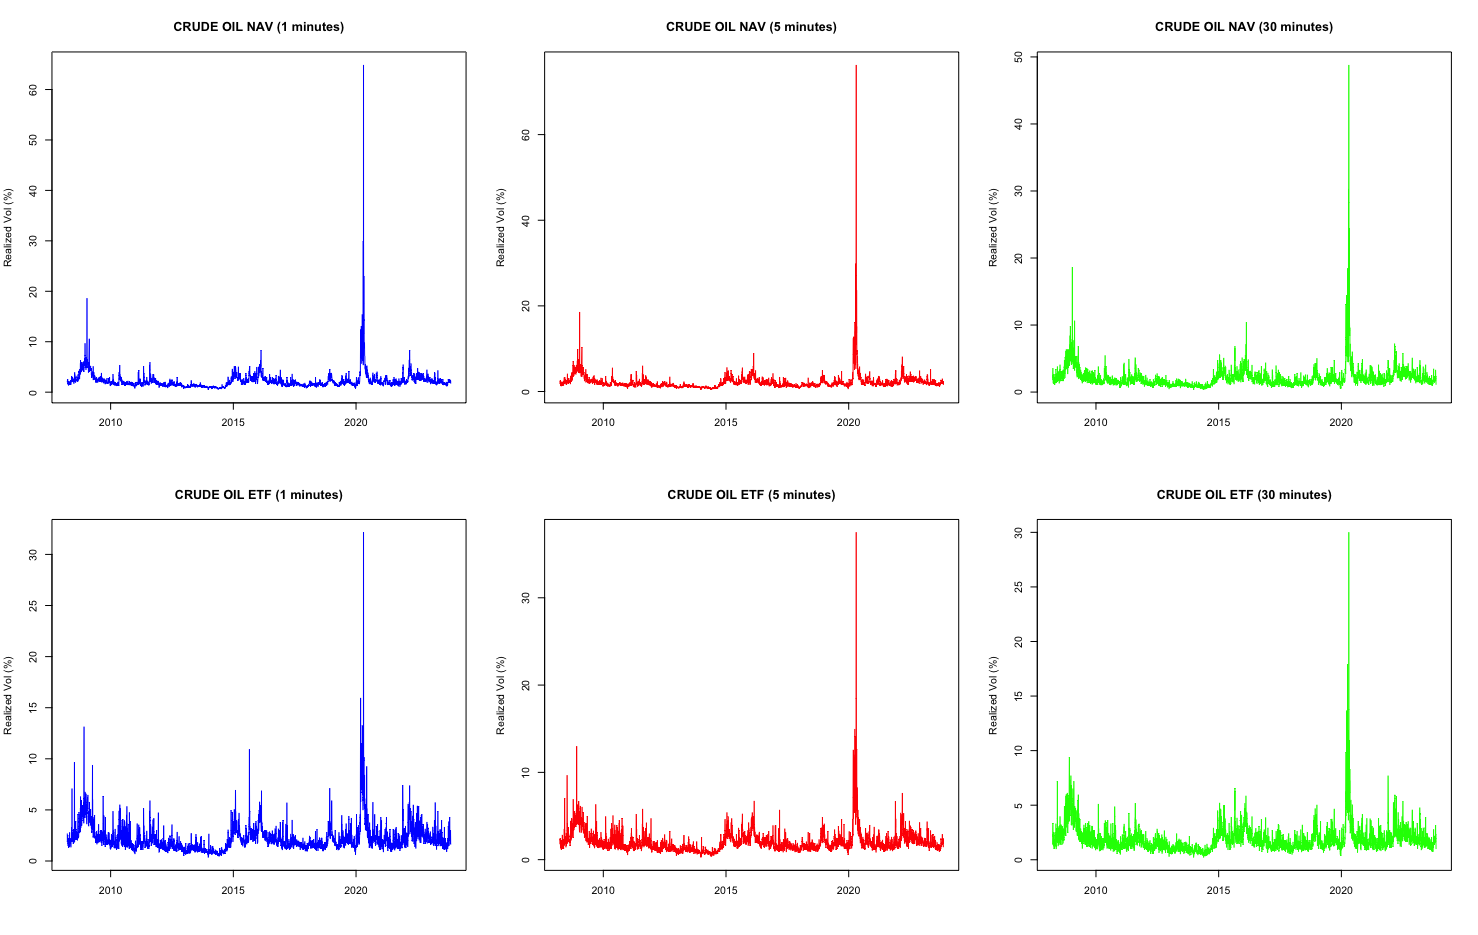
\includegraphics[width=16cm]{USO.png}
\centering
\caption{Realized Volatility for Crude Oil (ETF and NAV)}
\label{fig:rv_uso}
\end{figure}
\end{landscape}

\begin{landscape}
\begin{figure}[t]
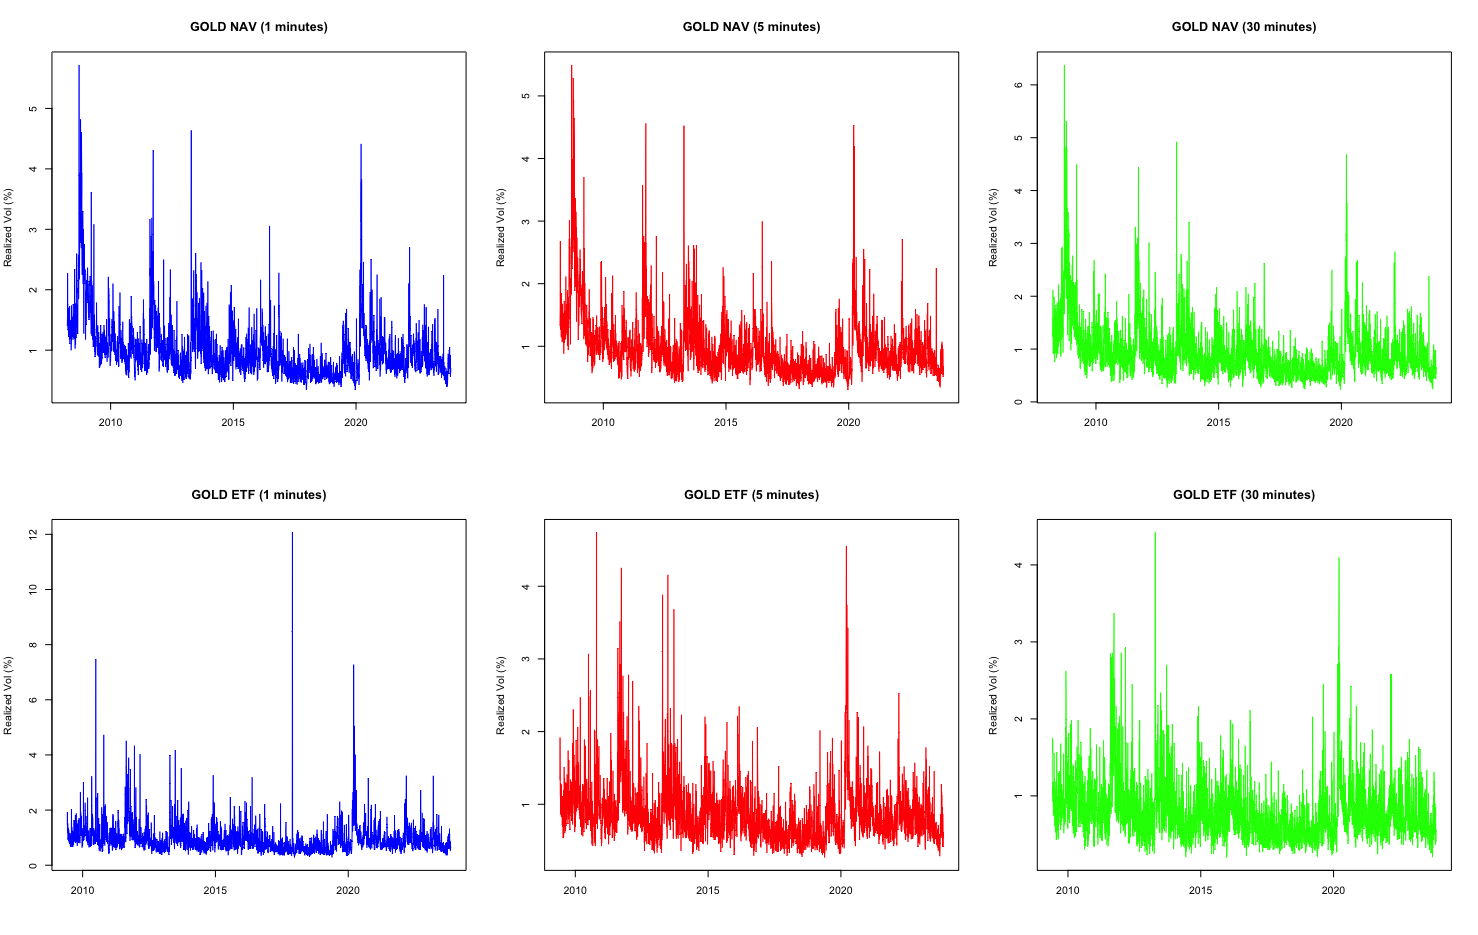
\includegraphics[width=16cm]{GLD.png}
\centering
\caption{Realized Volatility for Gold (ETF and NAV)}
\label{fig:rv_gld}
\end{figure}
\end{landscape}

\begin{landscape}
\begin{figure}[t]
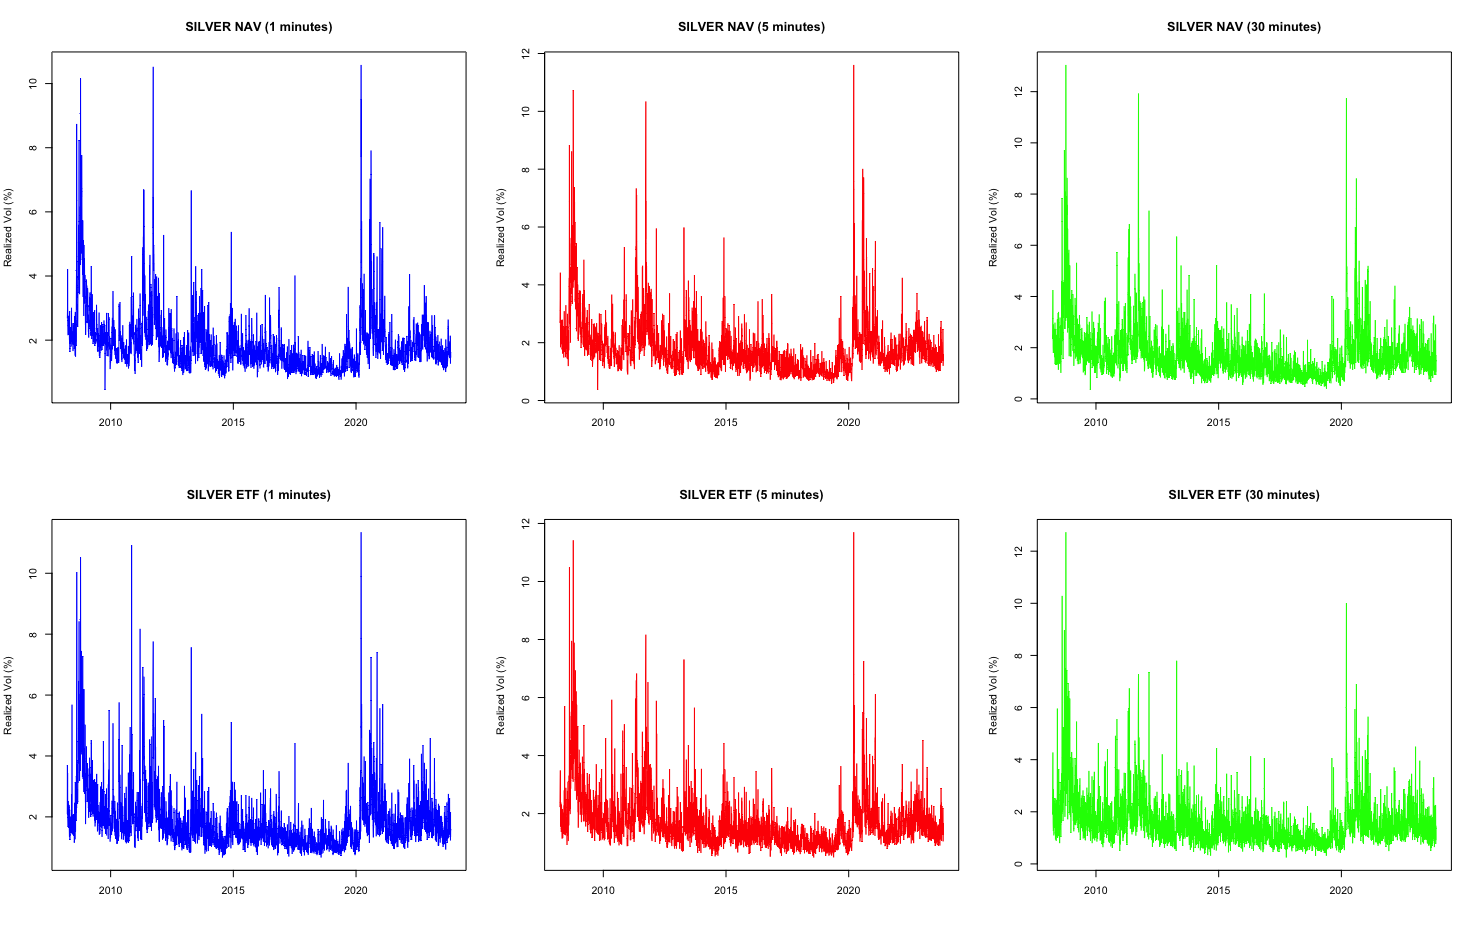
\includegraphics[width=16cm]{SLV.png}
\centering
\caption{Realized Volatility for Silver (ETF and NAV)}
\label{fig:rv_slv}
\end{figure}
\end{landscape}

\begin{landscape}
\begin{figure}[t]
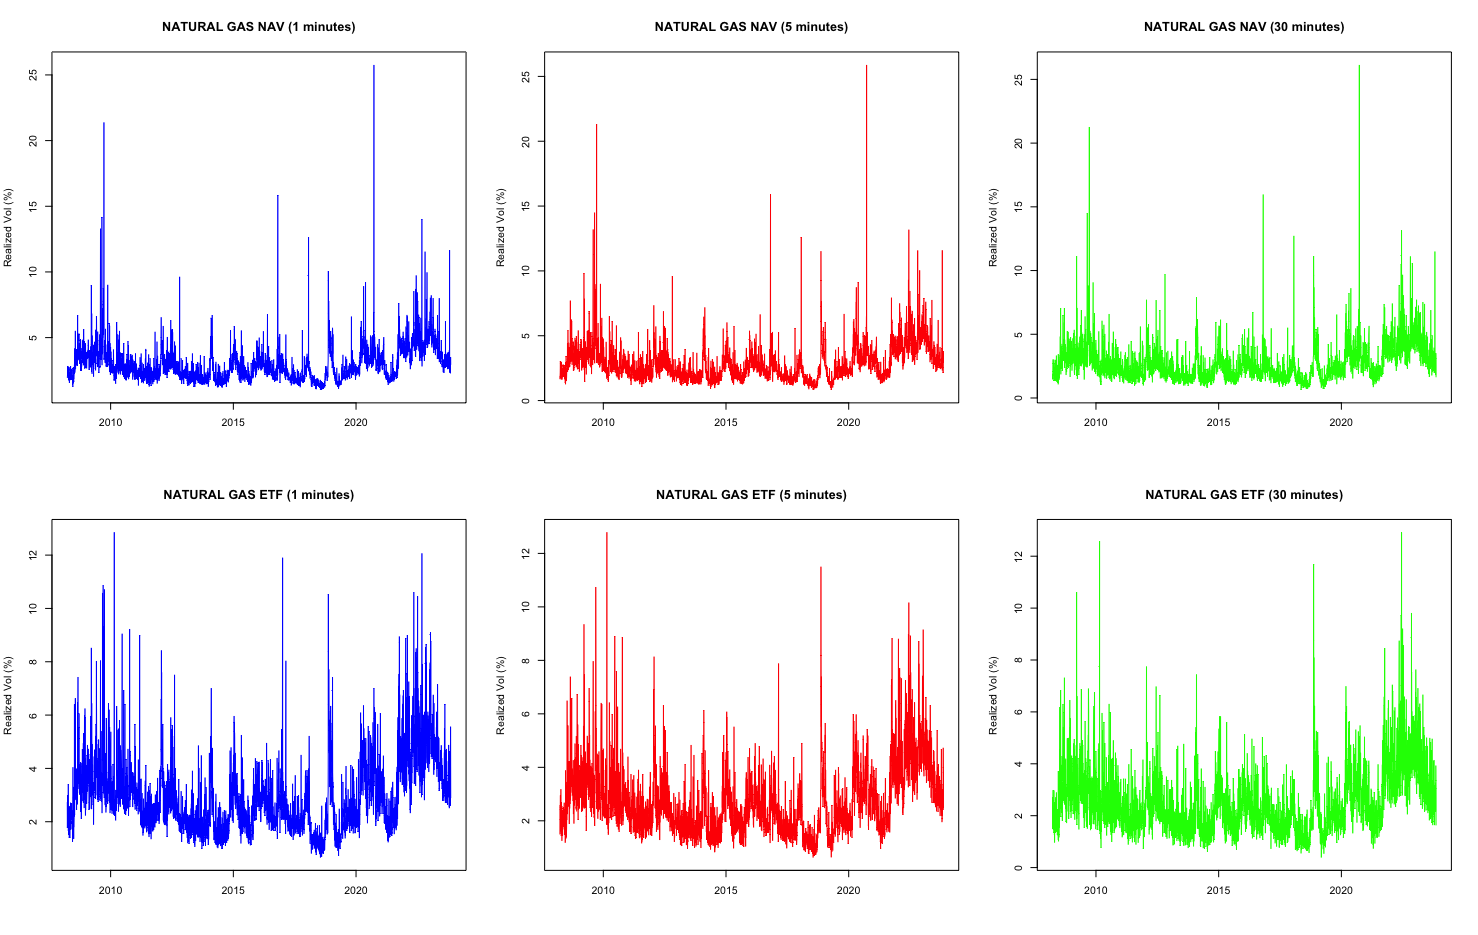
\includegraphics[width=16cm]{UNG.png}
\centering
\caption{Realized Volatility for Natural Gas (ETF and NAV)}
\label{fig:rv_ung}
\end{figure}
\end{landscape}

\begin{landscape}
\begin{figure}[t]
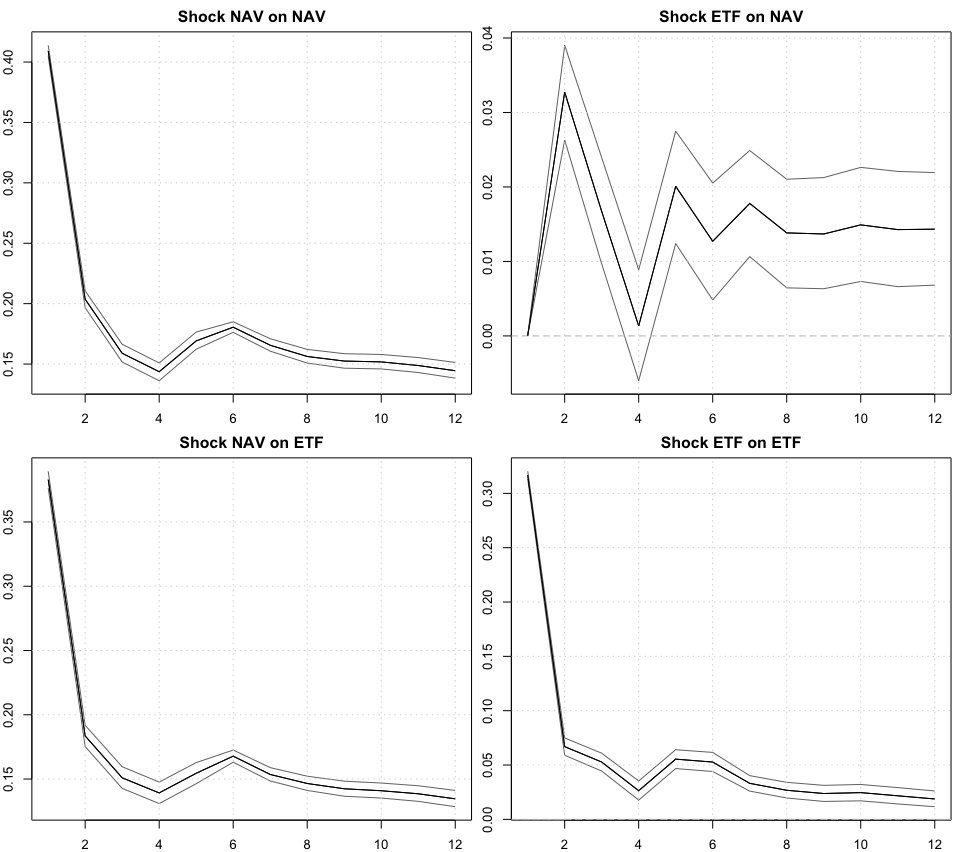
\includegraphics[width=16cm]{USO_irf.png}
\centering
\caption{Impulse Response Function (IRF) resulting from the modeling of the USO ETF and its Net Asset Value (NAV)}
\label{fig:irf1}
\end{figure}
\end{landscape}

\begin{landscape}
\begin{figure}[t]
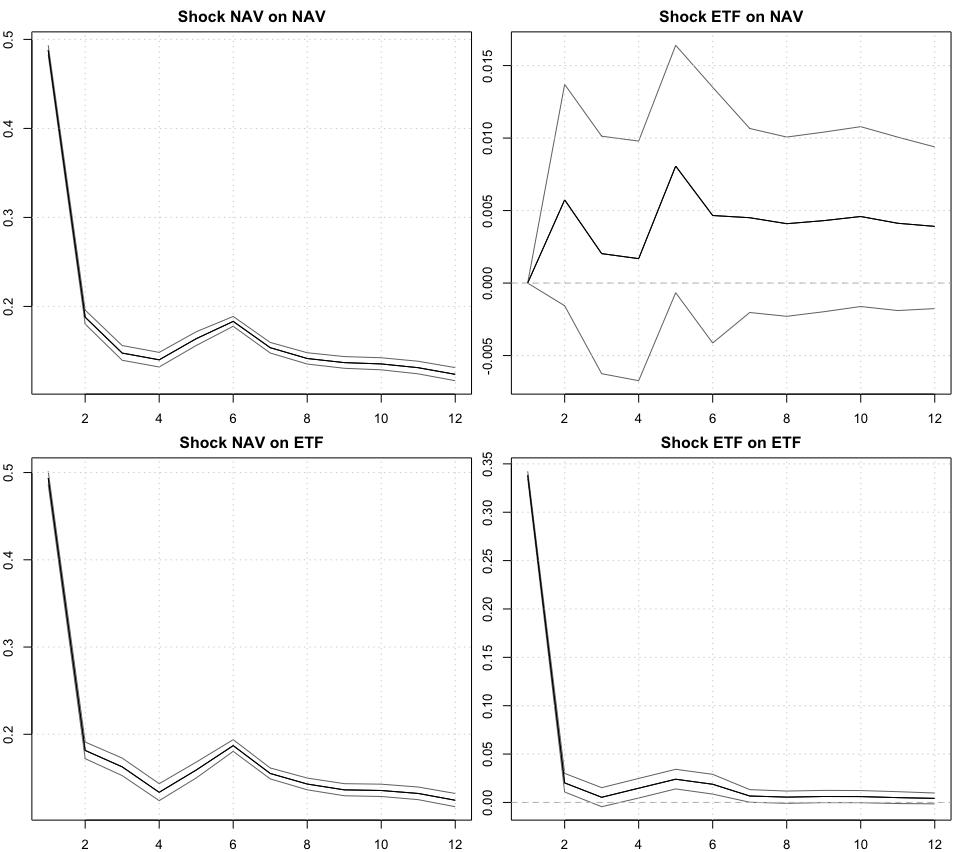
\includegraphics[width=16cm]{GLD_irf.png}
\centering
\caption{Impulse Response Function (IRF) resulting from the modeling of the GLD ETF and its Net Asset Value (NAV)}
\label{fig:irf2}
\end{figure}
\end{landscape}

\begin{landscape}
\begin{figure}[t]
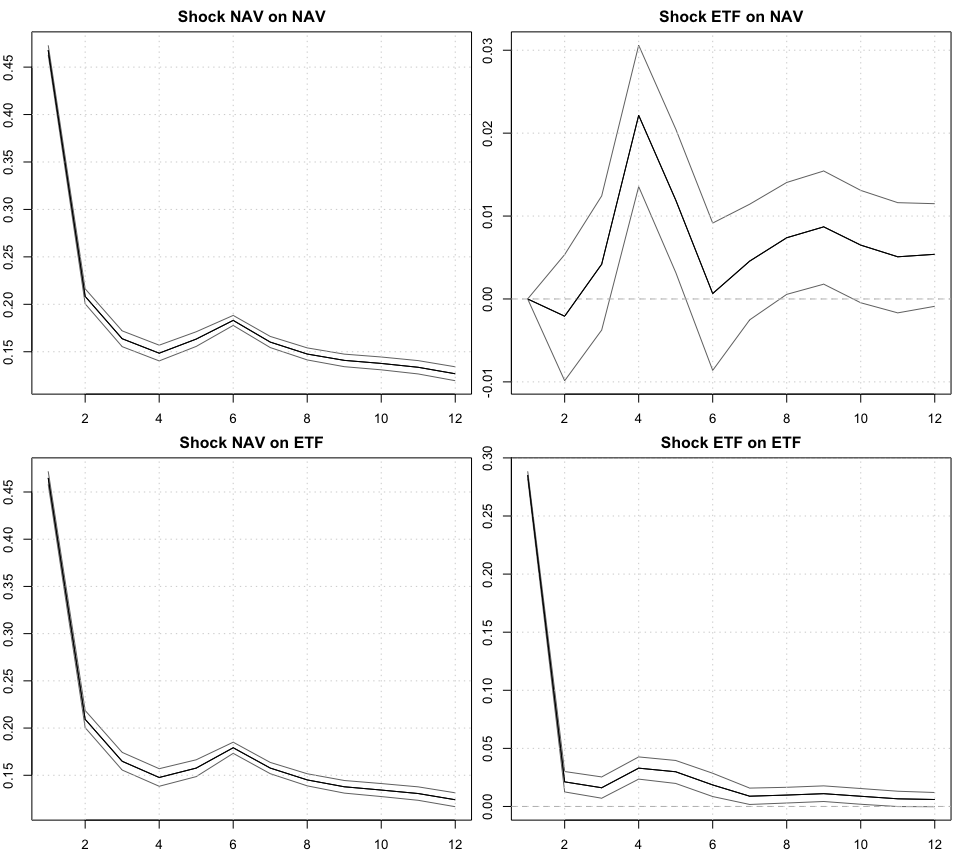
\includegraphics[width=16cm]{SLV_irf.png}
\centering
\caption{Impulse Response Function (IRF) resulting from the modeling of the SLV ETF and its Net Asset Value (NAV)}
\label{fig:irf3}
\end{figure}
\end{landscape}

\begin{landscape}
\begin{figure}[t]
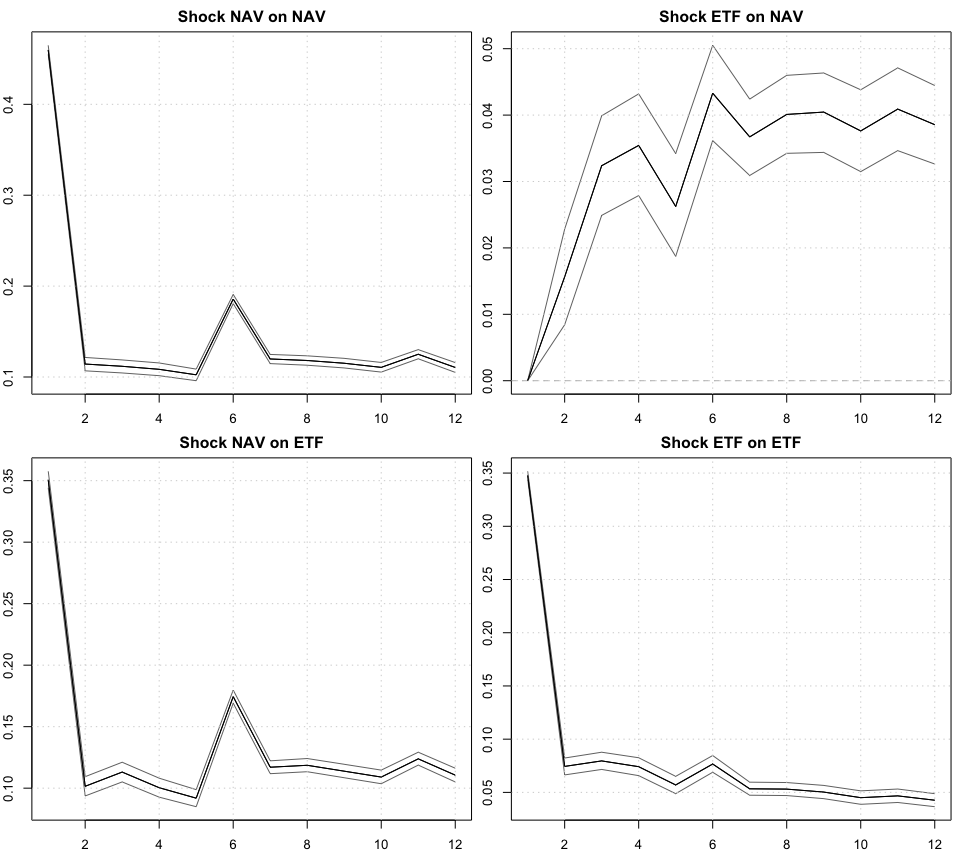
\includegraphics[width=16cm]{UNG_irf.png}
\centering
\caption{Impulse Response Function (IRF) resulting from the modeling of the UNG ETF and its Net Asset Value (NAV)}
\label{fig:irf4}
\end{figure}
\end{landscape}



\end{document}